% 논문 상신 결재 완결번호 : EP-2C15BBB05DF046F38F38EDD596390365
\documentclass[10pt,conference,letterpaper]{IEEEtran}
\IEEEoverridecommandlockouts
\usepackage{graphicx}
\usepackage[utf8]{inputenc}
\usepackage[hyphens]{url}
\usepackage[T1]{fontenc}
\usepackage[scaled=.8]{beramono}

% For table showing code
\usepackage{caption}

\usepackage{listings}

\usepackage{xcolor}

\lstset{basicstyle=\ttfamily,
  numbers=left,
  numbersep=5pt,
  showstringspaces=false,
  commentstyle=\color{red},
  keywordstyle=\color{blue}
}
% For parallel code blocks
\usepackage{fancyvrb}
% For enumerate with A. B. B., ..
\usepackage{enumerate}
% For more control in figure

\def\BibTeX{{\rm B\kern-.05em{\sc i\kern-.025em b}\kern-.08em
    T\kern-.1667em\lower.7ex\hbox{E}\kern-.125emX}}
\begin{document}


\title{Making Configurable and Unified Platform, \\
Ready for Broader Future Devices}

\author{\IEEEauthorblockN{MyungJoo Ham, Geunsik Lim}
%\author{\IEEEauthorblockN{Anonymized for double blind reviews}
\IEEEauthorblockA{\textit{Samsung Research, Samsung Electronics} \\
%\IEEEauthorblockA{\textit{} \\
Seoul, Republic of Korea \\
\{myungjoo.ham, geunsik.lim\}@samsung.com}
}
\maketitle

\begin{abstract}
The wide spread of IoT and edge devices has introduced new challenges for software platforms of consumer electronics, of which traditional targets had been smart phones, wearable devices, and smart TVs.
In general, such traditional devices share well-defined common features and requirements, which emerging IoT devices lack of.
Besides, IoT and edge devices have much longer tails, which makes it further intractable to define common features and requirements, composing a customized software platform.
Such high diversities prohibits having individual build configurations per device type, which multiplies burdens for developers as well as infrastructures.
Besides, IoT developers need to create customized platforms for new devices on-the-fly, which traditional platform tools are not capable of; such tasks usually require the rare release and build experts along with significant time and effort.
In this paper, We have successfully addressed the issues: unifying software platform (Tizen) and its infrastructure to increase the developmental productivity for varying device types and making Tizen highly configurable so that even third party developers may create their own variations on-the-fly easily and quickly.
This has enabled a public web service, \url{Craftroom.tizen.org}, where IoT developers may acquire their own customized Tizen on-the-fly.
This project is integrated into Tizen since 4.0, which is released to the public, and has enabled Tizen team to start IoT platforms and a small team to prepare software platforms for autonomous driving systems and on-device AI systems with minimal time and effort.
\end{abstract}

\begin{IEEEkeywords}
software engineering, build system, release and deployment, software platform
\end{IEEEkeywords}

\section{Introduction}\label{S_intro}
Traditionally, software platforms for consumer electronics (e.g., Tizen, Android, and iOS) have clear target device profiles: phones, wearable devices, tablets, or TVs.
Such a profile defines common API sets, features, and requirements across different products of the profile.
However, the wide spread of IoT and edge devices has introduced a new challenge: the long tail of the IoT~\cite{1Want2015EnablingTI}, which, in turn, incurs following significant challenges to software platforms:
\begin{itemize}
\item Each IoT device might require its own customized software platform: \textit{configurability}.
\item Even with a shared source code repository, various software platforms are built with different configurations, incurring extremely high build workloads: \textit{build explosion}.
\end{itemize}


Both challenges have already incurred significant developmental costs with traditional smart devices.
\textit{Build explosion} enforces developers and infrastructure to build and test software packages repeatedly for each profile.
Then, \textit{build explosion} attributes to the lack of \textit{configurability} by incurring high developmental costs to platform developers, which increase further with the long tail of the IoT.
Even if we have only 10 different IoT devices, not 100, we need to develop with 10 different build configurations for each commit and the build infrastructure suffers from additional x 10 workloads.
This is especially unacceptable with the long tail-ness; each IoT device type has little revenue although the whole IoT device portfolio may have huge revenue.
We cannot afford linearly increasing development costs with the increasing number of IoT device types.
Tizen platform developers have been already overloaded with the workloads multiplied by the number of profiles and suffered from the lengthy build task queues of the overloaded build infrastructure.
Thousands of build tasks had waited for several hours in task queues during busy hours despite of a lot of powerful build servers.


\textit{Configurability} is deteriorated not only by \textit{build explosion}, but also by the difficulties in composing a customized software platform with software packages.
There are well-established package management systems (e.g., Advanced Package Tool (APT) for DEB packages~\cite{blackman2000debian} and Zypper/DNF for RPM packages~\cite{foster2003red}), which allow to choose software packages without understanding inter-package dependencies.
However, developers still need to choose packages required by their software platform from the thousands of candidates, which require deep understandings of the software platform from device drivers and system software to applications.
Because such developers are rare, prototyping a lot of varying devices and their customized software platforms cannot be accomplished with the traditional and well-established tools.
Therefore, we need new tools that allow novice developers (developers without such deep understandings) to compose properly customized software platforms.


We address \textit{build explosion} first in order to enable \textit{configurability} because we should be able to build software packages for various devices with affordable workloads and to provide a single unified binary package repository of candidate packages to be chosen from.
We address \textit{build explosion} by unifying Tizen build procedures and binary repositories, enforcing every profile to share a single repository of binary packages, not only the source codes: Tizen:Unified project.
In order to unify Tizen, we introduce new rules for platform developers and plugin architectures with new dependency rules, enforced by build systems and Linux packaging systems, which are upstreamed to open source communities as well so that the new rules comply with the standard.
Thanks to the cooperation from platform developers and the communities, we have fully unified Tizen projects and repositories since Tizen 4.0 in 2017.


Unifying binary repositories mitigates the build workload not only for new IoT devices, but also for the traditional smart devices.
Tizen project (Tizen:Unified in \url{https://build.tizen.org}) no longer builds five times for five profiles, but builds only once for all device types, which is expected to reduce the workload of infrastructure roughly to one fifth.
With Tizen:Unified, peak build task waiting queue size has dropped from thousands to tens \cite{2Ham2017TDC}.


This work applies new infrastructure designed to promote \textit{configurability} along with Building Blocks of Tizen after Tizen:Unified.
Building Block definitions~\cite{3TizenWikiBB,4LeeKeynote2017TDC} provide easy-to-configure components to build a customized software platform maintained by product managers.
Building Blocks are meta packages with hierarchical structures that provide easy-to-understand descriptions.
A Building Block, existing as an RPM package, does contain any files, but has relational information of software packages and other Building Blocks; thus, it is a meta package.
Tizen Image Creator (TIC)~\cite{2Ham2017TDC} offers a web user interface to compose a software platform with Building Blocks and individual packages.
Tizen also offers a public web service for novice IoT developers, Craftroom~\cite{5CraftroomURL}, a simplified and beautified variation of TIC.
TIC and Craftroom provide new customized software platforms for IoT developers within minutes, not hours or days.


We design and implement both projects, Tizen:Unified and Tizen:Configurability, refactor software packages, restructure build procedures and rules, which enables on-the-fly platform customization.
Build and packaging rules introduced in this work are either within the Linux standard (RedHat/OpenSUSE) or upstreamed to the community.
This work significantly reduces build and test workloads of conventional devices and enables Tizen for wider ranges of device types with significantly reduced workloads of both developers and infrastructure.
This work is applied to Tizen 4.0 (2017) and 5.x (2018/2019), enabling various new products and prototypes, ranging from home appliances and IoT prototypes to autonomous driving systems and on-device AI platforms.

\section{Related Work}\label{S_related}
%%%%%%%%%%%% WIP. Needs extensie rephrases!!!!!

\subsection{Linux package management}

% Add a short summary for this subsection
A modern software platform has extremely large number of packages with complex inter-package dependencies, which is partially induced by shared libraries and daemon services complicating dependencies and dividing packages into smaller packages.
As a result, modern Linux package management system is required to manage complex inter-package dependencies consistently and efficiently.


\textit{Mancinelli et al.}~\cite{11Mancinelli2006ASE} have proposed to handle dependencies between packages automatically.
Most of its prior approaches have focused on declaring forward dependencies (i.e., \texttt{Requires} or \texttt{BuildRequires} in RPM systems) and following them.
This work~\cite{11Mancinelli2006ASE} tries to automatically discover undeclared dependencies by inspecting build scripts.
Caixa Magica and Mandriva Linux distributions use this method.


%%%%%%%%%%%% WIP. Needs extensie rephrases!!!!! CANNOT UNDERSTAND!
Requirements for future software build systems including choices, benefits, and challenges of a well-designed build process are described in~\cite{12Smith2011SBSBook}.
It surveys the tools and techniques for building software and how things may go wrong.
They conjecture that inadequate build systems can dramatically deteriorate the productivity; a subpar build system may incur bad dependencies, false compile errors, failed software images, slow compilation, and excessive labors.
It explains how to increase the performance and scalability of a build system. 


%%%%%%%%%%%% WIP. Needs extensie rephrases!!!!! CANNOT UNDERSTAND!
\textit{Galindo et al.}~\cite{13Galindo2010DebianPR} suggest realistic variability models to evaluate dependencies, a major and traditional problem of Linux communities.
They suggest that the package dependency language of Debian is a variability language and provide a mapping from the language to propositional formulas analyzing dependencies with SAT solvers.
They address other variability dependency languages of open source communities as well, which increases the availability of realistic variability models up to 20,000 packages for the Software Product Line community.
However, they do not detect anomalies as conditionally dead packages or redundancies.


\textit{Cosmo et al.}~\cite{14DiCosmo2008PUF} point out why the upgrade problems faced by Free and Open Source Software (FOSS) distributions have characteristics not easily found elsewhere.
They provide periodic snapshots of a whole software platform, which can mitigate OS upgrade problems along with disk partitioning.
They survey current countermeasures to such upgrade failures, argue that they are not satisfactory, and sketch alternative solutions.
They focus only on applying fingerprinting techniques to cluster maintainer scripts of Debian distribution to get a clear view of all their use cases.


\textit{Adoption of Academic Tools}~\cite{15abate2017debian} presents an overview of 10 years of research in this field and the process leading to the adoption of our tools in a FOSS community.
They presented the check tools such as \textit{distcheck} and \textit{buildcheck}, which scan all the packages in a Debian distribution to identify installability issues.
They focused on the Debian distribution and in particular they looked at the issues arising during the distribution lifecycle: ensuring buildability of source packages, detecting packages that cannot be installed and bootstrapping the distribution on a new architecture. 


\textit{Schroeder}~\cite{16Schroeder2007SatSolverURL} depicts the package dependency solver library that is called SAT solver.
This project has been started in May 2007 when the ZYpp community has decided to use a database to speed up installation.
It offers an efficient file and memory representation for complex dependency relations and package repositories.
The SAT solver of Libzypper is a port from the red carpet solver, which is to update packages of a running system.
In addition to SAT solver, they provide ad-hoc mechanisms to discover some of undeclared dependencies and an audit function for weak dependencies.


\textit{Zypper}~\cite{20Zypper_URL} is a package manager that installs, updates, and removes packages and manages repositories.
It is especially useful for managing software packages remotely or with shell scripts.
With Zypper, we can easily update the distribution.
Besides, we can update the software platform in run-time.
Note that Tizen is fully compatible with Zypper although it is not included in most traditional Tizen profiles.

\subsection{Build systems of Tizen}

% Add a short summary for this subsection
We describe build and release systems of Tizen, a software platform for IoT/edge devices, general consumer electronics, mobile phones, wearable devices, or even autonomous driving vehicles.
The standard packaging for Tizen is RPM~\cite{foster2003red}, which is also standard for OpenSUSE, RedHat, and Fedora.
We do not discuss Debian packages~\cite{blackman2000debian} although it is one of the two major standards along with RPM in Linux communities.
Note that the expression power of inter-package dependencies of Debian is not higher than that of RPM; Debian package dependencies may be expressed with RPM dependencies.

\textit{Git Build System (GBS)}~\cite{17GBS2014TizenURL} is a build and packaging tool for Tizen platform development.
It generates tarballs, builds sources, and packages binaries from Git repositories.
GBS also does local unit tests, provides build and test sandboxes, submits code to the build infrastructure, OBS.
Package maintainers may use GBS to maintain their upstream branches or forks, or to prototype packages not included in Tizen mainline.


\textit{MIC Image Creator (MIC, originated from Meego Image Creator)}~\cite{18MIC2014TizenURL} builds software platform images for Tizen.
MIC creates images of different types, including live CD images, live USB images, raw images for KVM~\cite{21Kivity07kvm}, loop images for IVI platforms, and filesystem images for chrooting.
Users can enter into the generated images with MIC. MIC changes the apparent root directory with a \textit{chroot} mechanism for the current running processes.
Note that MIC uses Zypper~\cite{20Zypper_URL} to resolve package dependencies during image creation.


\textit{Open Build Service (OBS)}~\cite{19OBS_URL} is a general build, release, and distribution system for various target platforms in an automatic, consistent, distributed, and reproducible way.
OBS releases software for a wide range of operating systems and hardware architectures with extensible web interfaces and APIs.
It is an open and complete distribution development platform that provides a transparent infrastructure for the development of Linux distributions, used by openSUSE and Tizen.
OBS supports Fedora, Debian, Ubuntu, RedHat, and many distributions.
Like GBS, OBS builds binaries in a sandbox to ensure the consistency.
OBS may create binary packages in varying formats including RPM~\cite{22foster2002red}, DEB, and many others.
The created packages can be released and deployed via repositories compatible with package managers.




\section{Issues of Tizen before 4.0}\label{S_IssueBefore4}

Tizen before 4.0 has a build project for each profile: i.e., Mobile, Wearable, TV, IVI, and Common, which has its own binary repository.
Such binary repositories are not disjoint; there are packages with duplicated names across profiles.
Thus, we cannot compose a software platform with packages of different profiles because the inter-package dependency chain of a profile is not compatible with that of others.
For example, with packages \texttt{A}, \texttt{B}, and \texttt{C}, present in all profiles, where \texttt{A} and \texttt{B} depends on \texttt{C}, we cannot install \texttt{A} from Mobile and \texttt{B} from TV because we cannot install two instances of \texttt{C} from both profiles.
Note that Common profile is simply yet another profile and does not represent common part of others.


Creating a new device type, which happens very frequently with IoT and edge devices, has required to define a new profile and its dedicated build project.
This is not a unique issue of Tizen; Android, dominant for mobile phones, and Yocto~\cite{Streif:2016:ELS:3051933}, popular for IoT devices, also require an independent build project for each device prototype.
For each build project, the infrastructure is required to build the whole packages and developers are required to build and test the packages.
This incurs redundant workloads proportional to the number of device types.
Even if the same source codes are shared across profiles, the whole packages are built repeatedly, which is already too expensive with only five profiles.


Frequently prototyping new device types significantly multiplies such workloads, making it intractable.
Administrators do not allow creating new profiles in the already overloaded infrastructure, where developers and managers keep complaining about the latency.
Besides, creating a new profile has been too difficult for non-build-expert developers.
It requires to fully understand low-level system software packages and the underlying mechanisms of build systems.


\section{Design of Tizen:Unified}\label{S_ach_build_unif}

We have achieved the unification in April, 2017.
We have removed per-profile build projects and provided a single build project and binary repository for all.
The objectives of the unification includes: a) shorter build latency by eliminating duplicated builds; thus, making affordable to support more profiles, b) allowing to create arbitrary profiles from a single shared binary repository, and as a results of a) and b), c) allowing to create new profiles on-the-fly without rebuilding packages, enabling the next big step, configurable Tizen.


There are two major rules to achieve the unification:
\begin{itemize}
\item In build-time, build processes (build scripts, compilers, and build systems including OBS~\cite{19OBS_URL} and GBS~\cite{17GBS2014TizenURL}) should be agnostic to the profile except for the architecture: e.g., \textit{armv7l} and \textit{x86\_64}.
However, processes may identify the profile at install-time, boot-time, or run-time.
\item Every single binary package (i.e., RPM for Tizen) should be able to co-exist in a single repository with other packages as long as the packages have the same architecture.
\end{itemize}

With the completion of the unification, these rules have been applied for all Tizen packages.
The build system is configured to enforce the rules automatically so that any violating changes cannot affect the system since Tizen 4.0~\cite{2Ham2017TDC}.


For the unification, the huge number of software packages itself has been a significant challenge; e.g., Tizen 3.0 Common profile has 822 source packages~\cite{2Ham2017TDC}.
When we have started planning Tizen:Unified in July, 2016, we have discovered 134 source packages disobeying the rules.
When we have started refactoring with a small team of four developers in November, 2016, the number of such packages has increased to 171.
Another challenge is the regression, where a complying package becomes not complying.
We have observed multiple cases of such regressions, both regressions of the refactored packages and natively complying packages.


Ideally, refactoring is better executed by main contributors of the package.
However, it requires the main contributors to fully understand the concept of Tizen:Unified, the mechanisms of build systems under their own workloads and tight schedules.
During the early phase of the project, as a pilot program, we have tried the ideal method with few small groups.
As the result, we have learned the following points:


\begin{itemize}
\item We should not expect developers to fully understand the build system and inter-package dependencies.
They are users of the build system and a good build system should not require users to understand the system itself.
\item It is extremely difficult to ensure that the rules are kept during active development where new commits are applied daily if not hourly.
\item Applying yet another coding rule requires additional burden to developers.
Even if the need is justified to team leaders and main contributors, it is often not enough for them to put additional efforts to prevent others from breaking the rules or to review more carefully.
Moreover, we cannot enforce the rules with the infrastructure until every package follows the rule perfectly because any disobeying package will break the build.
\end{itemize}

As a conclusion, we have decided to do all the refactoring with Tizen:Unified members except for a few packages (Chromium, EFL, and input systems) with much complicated issues that require to rely on their own main contributors.
During the progress of Tizen:Unified project, to detect any attempts of regression, we have developed a gerrit~\cite{6GerritURL} monitoring service that reviews incoming commits and finds any possible regressions.


We categorize packages to refactor into the following types:
\begin{itemize}
\item \textbf{Type-A.} The build script is aware of profiles. It may use different source files or code blocks statically (usually with \texttt{\#ifdef} or \texttt{\#if}) per the profile.
\item \textbf{Type-B.} Multiple git repositories generate packages with a common name. For example, both \texttt{mobile/efl-config.git} and \texttt{wearable/efl-config.git} had generated efl-config.
\item \textbf{Type-C.} At build-time, the package depends on packages that generates different build environments per profile.
\end{itemize}

We have observed a lot of useless dependencies on the profiles or device types and removed them immediately.
We also have had cases where the dependencies are easily removed by using configuration files in \texttt{/etc}. 


\subsection{Runtime profile identification}\label{SS_RUntimeProfileId}

If we cannot avoid per-profile behaviors, applying the runtime profile identification is recommended.
This is recommended because it allows using the same binary across different profiles avoiding installing different binaries per profile.
The only more recommendable method is to behave exactly same regardless of the profile definition itself, which is often impossible.
Many Type-A cases are resolved by this.

\renewcommand{\tablename}{Code}
%% TODO : Check the template if this is allowed.
\begin{table}

\begin{center}
\line(1, 0){250}
\end{center}
\vspace{-0.1cm}

\hspace{0.5cm}\begin{BVerbatim}[baseline=c]
#ifdef PROFILE_MOBILE
    Do_mobile_action();
#else
    Do_common_action();
#endif
          (a)
\end{BVerbatim}
%% \quad$\parallel$\quad
\begin{BVerbatim}[baseline=c]
  ||  if (get_profile() == MOBILE)
  ||      Do_mobile_action();
  ||  else
  ||      Do_common_action();
  ||       
  ||            (b)
\end{BVerbatim}

\vspace{-0.1cm}
\begin{center}
\line(1, 0){250}
\end{center}
\vspace{-0.2cm}

\captionsetup{labelformat=simple,labelsep=period}
\caption{(a) Type-A code with \texttt{\#ifdef} and (b) refactored code}\label{TABLE_CODE_IFDEF}
\end{table}

In order to allow runtime identification, we have used a Tizen API to detect the profile and removed all preprocessor conditionals related. Code~\ref{TABLE_CODE_IFDEF} shows a simple example where such refactoring is applicable.

\subsection{Inter-package dependency management}\label{SS_interpkg_dep_mgt}

Sometimes, we have created different binary packages for each profile or device types along with meta packages or virtual packages (RPM capabilities) to make per-profile differences transparent to other packages.


Let us assume that we have a package \textit{X}, which needs to have different binaries for mobile profile.
Then, we can write the build scripts to create a subpackage, \textit{X-profile\_mobile.rpm}.
The first variation of the mechanism is to create \textit{X.rpm} file for other profiles and to create \textit{X-profile\_mobile.rpm} that may act as \textit{X.rpm} by adding the reverse-dependency, \textit{Provides: X}.
With the first variation, \textit{X.rpm} needs to declare that it \texttt{Provides} virtual subpackages such as \textit{X-profile\_common} in order to be explicit for per-profile configurations.
The second variation is to create a meta package, \textit{X.rpm} without any files, but with meta data stating its dependencies on a virtual subpackage, \textit{X-compat}, and to create subpackages of profiles that do \texttt{Provides: X-compat}, which enforces to install one of such subpackages to install \textit{X.rpm}.
Both variations require subpackages to declare \textit{Conflict} statements to prevent installing plugins of different profiles for one main package.


A critical side effect of these mechanisms is that build systems (both OBS~\cite{19OBS_URL} and GBS~\cite{2Ham2017TDC}) are confused by multiple candidates (the subpackages) for inter-package dependency resolutions.
In other words, if \textit{X.rpm} is required by \textit{Y.rpm} while we build \textit{Y.rpm}, the build systems cannot determine whether it should install \textit{X-profile\_mobile.rpm} or the other; they do not accept such ambiguity.
We have resolved such ambiguity with weak dependencies, \texttt{Recommends}, to declare default selection for build systems, which the corresponding open source community (BSSolve and OBS) have accepted.
We have chosen the weak dependency, \texttt{Recommends}, because we can override it with strong dependency, \texttt{Requires}, for other plugins or profile supports while we may provide hints for build systems.
There is a weaker dependency in RPM standards, \texttt{Suggests}; however, we have not used it for this purpose because only human is supposed to use \texttt{Suggests}; thus, we use \texttt{Suggests} for constructing package list GUI only.
Note that having the default package with \texttt{Recommends} at built time does not affect software platforms with different plugin packages because they are shared objects; only their forms (header files) matter, which holds for Tizen native platform binaries.
However, we had exceptions to this, mentioned in the next section, where the contents of external headers (APIs) differ per profile.



\begin{figure}
\centering
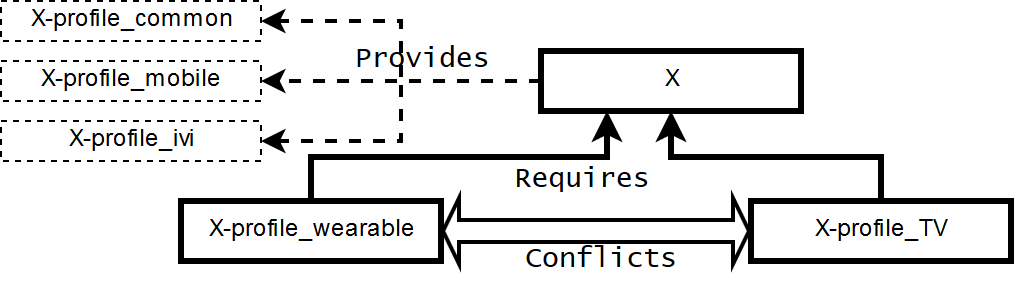
\includegraphics[width=0.98\columnwidth]{figures/Dependency_nonmeta_X.png}
  
\vspace{0.2cm}
  
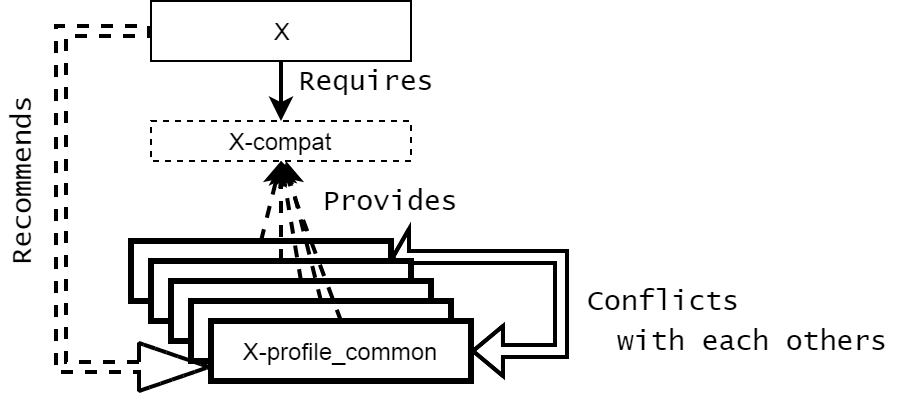
\includegraphics[width=0.98\columnwidth]{figures/Dependency_metaX.png}
% For more control in figure
\caption{The two subpackaging examples supporting different binaries per profile transparently to other packages.}
\label{FIG_TZN_TYPEB_RESOL}
\end{figure}

Fig.~\ref{FIG_TZN_TYPEB_RESOL} elaborates inter-subpackage dependency management mechanism; the top shows the first variation and the bottom shows the second variation.
Note that any packages external to \textit{X} should not explicitly depend on profile plugin subpackages (\textit{*-profile\_*.rpm}).
Such packages should refer to the main package (\textit{X} in Fig.~\ref{FIG_TZN_TYPEB_RESOL}) only and let the package management system handle the rest.


Type-B and Type-C are mostly resolved by declaring inter-package dependencies explicitly after properly refactoring the build scripts and source codes so that per-profile parts are separated into different binary packages.
There are many Type-A cases resolved by this mechanism as well when it is too difficult to apply the mechanism of the Section \ref{SS_RUntimeProfileId}.
It is usually when a profile has completely different source code files, which incurs too large modifications to apply runtime profile identifications.
In such cases of Type-A, we generated different executables for each profile and packaged them into different binary packages, which is often referred as sub packages.
However, for the package management mechanism, there are no differences between packages and sub packages.


\subsection{Inappropriate definitions of APIs}\label{SS_uglyAPI}

Unfortunately, a few developers have written external header files with different function declarations per profile or even provided different header files for different profiles.
There has been even a case where Tizen public API header has different C enum definitions per profile.
In this case, the C enum definitions of mobile have been \texttt{PLAYER\_DISPLAY\_TYPE\_EVAS = 1} and \texttt{PLAYER\_DISPLAY\_TYPE\_NONE = 2} while those of wearable have been \texttt{PLAYER\_DISPLAY\_TYPE\_EVAS = 2} and \texttt{PLAYER\_DISPLAY\_TYPE\_NONE = 1}.
This extreme case has required Tizen public API changes that may make previous applications incompatible with new Tizen versions.
Thus, we have redefined C enum values with unused and unified values and marked old values (1 and 2) as deprecated along with compatibility resolving code that behaves differently for each profile detected in run-time.


For the first case, where profiles have had different function declarations using compiler preprocessor conditionals, we have manually refactored header files removing all preprocessor conditionals.
We cannot apply the mechanism of Section \ref{SS_interpkg_dep_mgt} for headers exposed externally because the depending package (\texttt{X.rpm} in the examples of Section \ref{SS_interpkg_dep_mgt}) cannot be identical for different profiles; profile dependency is no more transparent to external packages!
For the other cases, where different files have been used per profile, we have manually inspected each declaration and merged them into a superset containing all declarations from all profiles.
Then, we have added dummy function definitions for profiles that do not or cannot execute it, determined either at run-time with profile probing APIs or at install-time with different binaries per profile.


\subsection{Workarounds}

There are a few cases where we cannot completely remove the dependencies on profiles or device types from the binary packages except for the plugin subpackages, which do not incur external dependencies.

\begin{itemize}
\item Case 1: Device drivers or kernel binaries require dependencies on device types and often, such dependencies are hardcoded.
\item Case 2: We are not allowed to generalize product or business division specific routines. A business division has required keeping their product specific conditional codes embedded in Tizen while such codes cannot be generally used for other profiles or devices. Although, in principle, this is undesirable as it fragments the source code and damages the readability, this has been something we could not alter.
\end{itemize}

Case 1 includes Linux kernel, which is built and installed for all devices, but their source code repositories or build configuration might differ.
We have applied an altered method of Section \ref{SS_interpkg_dep_mgt} as shown in Fig.~\ref{FIG_TZN_KERNELDEP}.


\begin{figure}
\centering
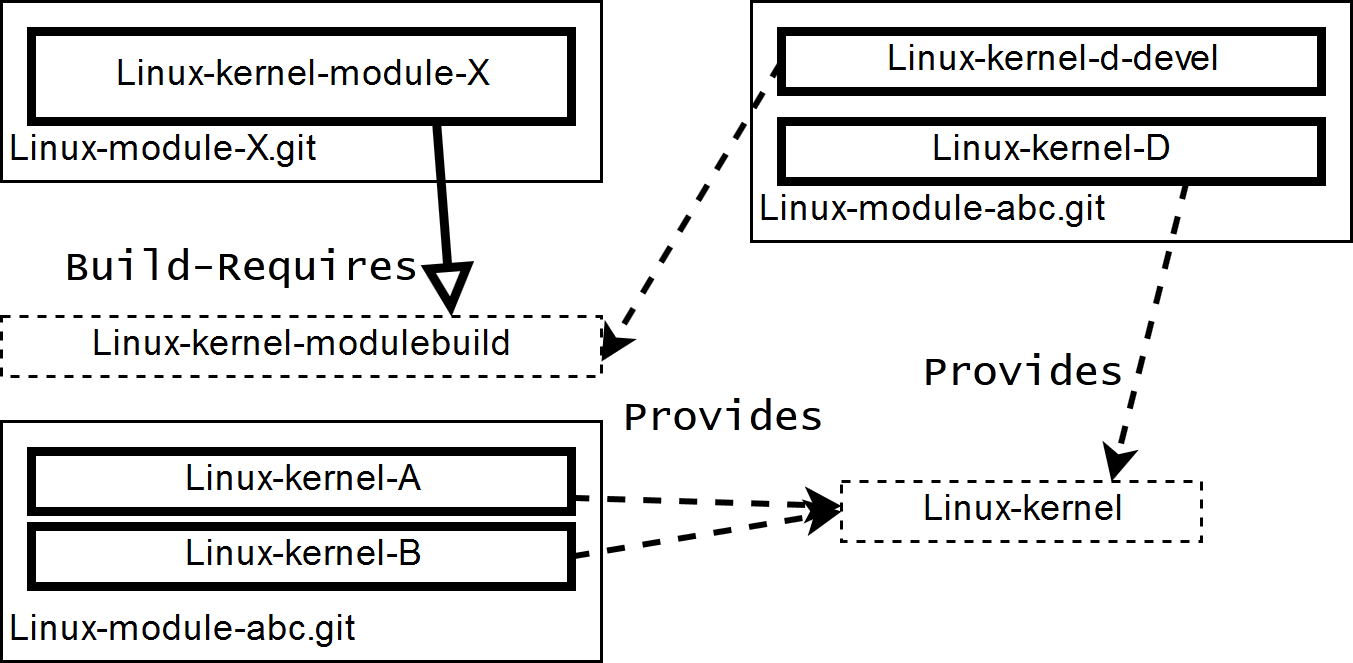
\includegraphics[width=0.95\columnwidth]{figures/KernelDeps_v2.png}
\caption{The altered method of Fig.~\ref{FIG_TZN_TYPEB_RESOL} for Linux kernel}
\label{FIG_TZN_KERNELDEP}
\end{figure}

As shown in Fig.~\ref{FIG_TZN_KERNELDEP}, different Linux kernel binaries from various git source repositories provide the capability of Linux-kernel so that any package or software platform manifests requiring Linux-kernel can be satisfied with one of Linux-kernel binary packages.
However, as mentioned before, we cannot have multiple candidates for a single dependency (or capability in RPM documents) in build time.
Thus, for external kernel module repositories, a representative kernel repository has been chosen to provide the Linux-kernel-modulebuild capability, which is the emulator kernel repository.
Note that we can have a single representative for each Linux kernel version.
Therefore, if there are multiple Linux kernel versions required for a specific Tizen version, we can choose multiple representatives, one for each kernel version.
We may choose multiple representatives without introducing the ambiguity for build systems by specifying kernel versions in kernel modulebuild dependencies.
That is \texttt{BuildRequires: linux-kernel-modulebuild = 4.4.0} and \texttt{Provides: linux-kernel-modulebuild = 4.4.0}  instead of \texttt{BuildRequires: linux-kernel-moduilebuild} and \texttt{Provides: linux-kernel-modulebuild}.


For case 2, we have configured the Tizen main public build systems to ignore any macros related with products or business divisions.
Although we have allowed preprocessor macro conditionals for products and business divisions, as long as the main build system ignores such macros, we can guarantee that the resulting binaries are complying Tizen:Unified.
Simultaneously, with the same source code repositories, a business division may keep their own special source code activated in their own build projects in their own private build systems.
However, codes creating different binaries under the same package names should be discouraged.
Such codes are usually the results of laziness (or overloaded workloads) of developers; they should have used configuration files (.ini files in /etc directory) or accessed Tizen device APIs, probing device type, name, and profiles.
We hope, in some day, such lame codes are totally eliminated.


\subsection{How we have progressed}

Regressions by incoming commits breaking the rules mentioned in the first paragraphs of Section \ref{S_ach_build_unif} have been headaches for the Tizen:Unified project.
Before April, 2017, during the active development of Tizen:Unified project, the build system could not be configured to ignore per-profile build configurations.
Thus, we have constantly monitored incoming Tizen commits with a monitoring service implemented to find any regressions in the rule enforcement.
For the reported regressions, we have intervened the related activities, where we could have successfully dropped or corrected violating commits before being merged.


Once every single package in Tizen has obeyed the given rules of Tizen:Unified, we have removed all per-profile build projects from the infrastructure and unified all Tizen packages into a single build project named \texttt{Tizen:Unified}, which does not allow any dependencies on profile or device types in built-time.
Note that build projects for older versions (e.g., Tizen 2.x or 3.0) are untouched and kept with per-profile basis; however, they are no more actively developed and do not require heavy build workloads as work-in-progress versions.
Another build project, \texttt{Tizen:Base} exists independently in order to reduce the performance impact from cyclic build dependencies of toolchains.
Cyclic build dependencies incur heavy redundant build workloads and are prohibited in Tizen:Unified because it is expected to be rebuilt frequently; most developers contribute to Tizen:Unified daily.
Note that as long as multiple build projects are disjoint (not sharing source repositories) and inter-project dependency is acyclic, there is no build performance problem and on-the-fly configurability.
The traditional per-profile build projects are not disjoint, sharing hundreds of source repositories with each other.


Once Tizen:Unified is completed, we have observed another unexpected advantage that we could have exploited for other projects.
We can add a disjoint build project that does not have cyclic inter-project dependencies without any deterioration on the performance or the configurability.
With this characteristics, we could have created aggressive prototypes quickly without affecting conventional Tizen projects.
An autonomous driving project and an on-device AI platform project require a lot of additional source repositories, well over 100.
Besides, although these projects are based on Tizen, they are not officially Tizen projects and the related packages could have not be included in official Tizen repositories.
By adding a disjoint build project, depending on Tizen:Unified, but outside of Tizen official build infrastructure, Tizen:TAOS (representing Tizen AI OS Support, Tizen Autonomous-driving OS, and Tensor-Aware OS simultaneously), we could have been aggressively prototyping new software platforms.
When there is a new need for yet another variation, a single developer can generate and deploy a new software platform and its binary images to corresponding developers and devices within few hours, which is frequently occurring.
The inter-project dependencies are shown in Fig.~\ref{FIG_TZN_INTERPDEP}.
In Fig.~\ref{FIG_TZN_INTERPDEP}, shaded blocks represent Building Blocks and white blocks represent individual software packages.
Blocks with thick outlines represent mandatory items--subblocks or individual packages of a block--, which means the items are chosen unconditionally if their parent is chosen.
For example, if a parent, \texttt{Graphics}, is chosen, its mandatory item (child), \texttt{2D}, is always chosen.
On the other hand, optional item, \texttt{3D}, is may be omitted even if \texttt{Graphics} is chosen.
Note that unless explicitly declared, a child may be chosen without choosing its parent.
For example, \texttt{3D} or \texttt{2D} may be chosen without choosing \texttt{Graphics}.
If the whole platform has not been unified as in pre-4.0 Tizen, this would have been challenging task because we cannot pick a few packages from a profile and some other packages from another profile simultaneously for a single new project.
Note that this is different from the configurability because the configurability is to configure a system within the official Tizen project.

\begin{figure}
\centering
  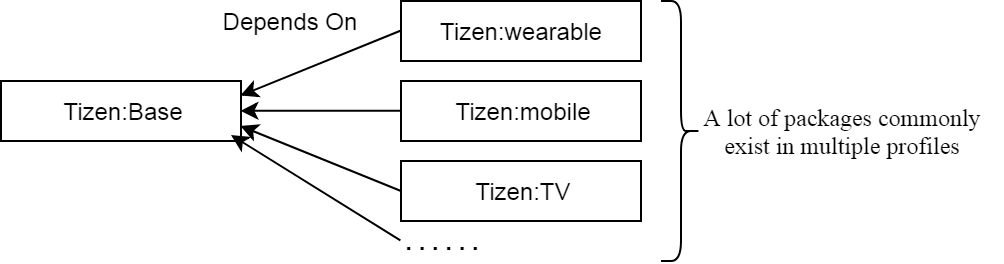
\includegraphics[width=0.95\columnwidth]{figures/InterprojectDeps_Old.png}
  
  \vspace{0.1cm}
  
  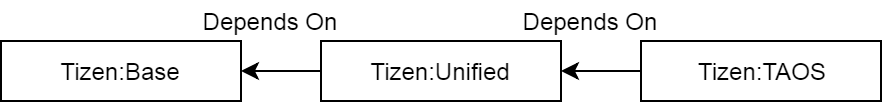
\includegraphics[width=0.85\columnwidth]{figures/InterprojectDeps_New.png}
\caption{Inter-project dependencies of Tizen build projects. The top shows pre-4.0 and the bottom shows 4.0 or later.}
\label{FIG_TZN_INTERPDEP}
\end{figure}

\section{Design of Tizen:Configurability}\label{S_Design_Tizen_Conf}

With the completion of Tizen:Unified project, Tizen has achieved the basic ability to configure a software platform on-the-fly.
Because every single binary package can be located in a single package repository and there is no more ambiguities between package names any more, we can now use package management systems without glitches anymore: zypper, DNF, or yum, which are equivalent to apt in Ubuntu/Debian systems.


For most workstations, PCs, or servers, this degree of configurability may be enough.
However, it is not enough for embedded systems and IoT/edge systems consisting of both devices and software platforms.
For such systems, we need to continuously release and deploy OS images that can be flashed to devices easily without manual labor.
Traditionally, in Tizen, we have been using a tool, MIC, previously named MeeGo Image Creator.
Issues with traditional tools include:

\begin{itemize}
\item Issue 1: It is too difficult to create a new software platform configuration (.ks file) for most users; you need build system experts who understand Tizen and its infrastructure deeply. Thus, it can be practically impossible for most third party developers to create Tizen prototypes.
\item Issue 2: You need your own dedicated Linux workstation to create Tizen images. It would be more appropriate if IoT application developers with an access to web browsers and Tizen Studio~\cite{23tizenstudio2018} can write their own IoT applications and generate proper Tizen OS images for their own IoT devices and applications on the fly.
\end{itemize}

In order to address Issue 1, we have introduced the concept of building blocks and implemented the first draft in \url{https://git.tizen.org/cgit/tools/building-blocks/} in May, 2017.
The concept of building blocks is now the core of Tizen profiles and device type definitions.
It is also the main tool for project managers.
With building blocks, users can create prototypes without the knowledge of thousands of individual Tizen packages or to choose hundreds from them, but with the fewer (about one or two dozens) abstract and easy-to-understand building block names: e.g., Bluetooth, Haptic, and Default-App-Setting.


In order to address Issue 2, we have introduced Tizen Image Creator (TIC), which has the web frontend with node.js.
Analyzing individual packages and generating deployable OS images for the configured prototype is executed in a web server.
Tizen team has opened web service that uses TIC and building blocks as its backend at \url{https://craftroom.tizen.org}: Craftroom.
Craftroom service offers simplified and easier interfaces focused on IoT developers.


\subsection{Building blocks}\label{SS_buildingblocks}

A building block is a meta packages that designates mandatory packages and optional packages.
As a meta package, it does not have its own files, but has dependency relation information consisting the list of mandatory or optional packages.
A mandatory package is an individual Tizen package or another build block that is installed if the corresponding building block is chosen.
An optional package is an individual Tizen package or another building block to be shown in the user interface if the corresponding building block is chosen.
Unlike mandatory packages, optional packages are not automatically chosen with the corresponding building block.


\begin{figure}
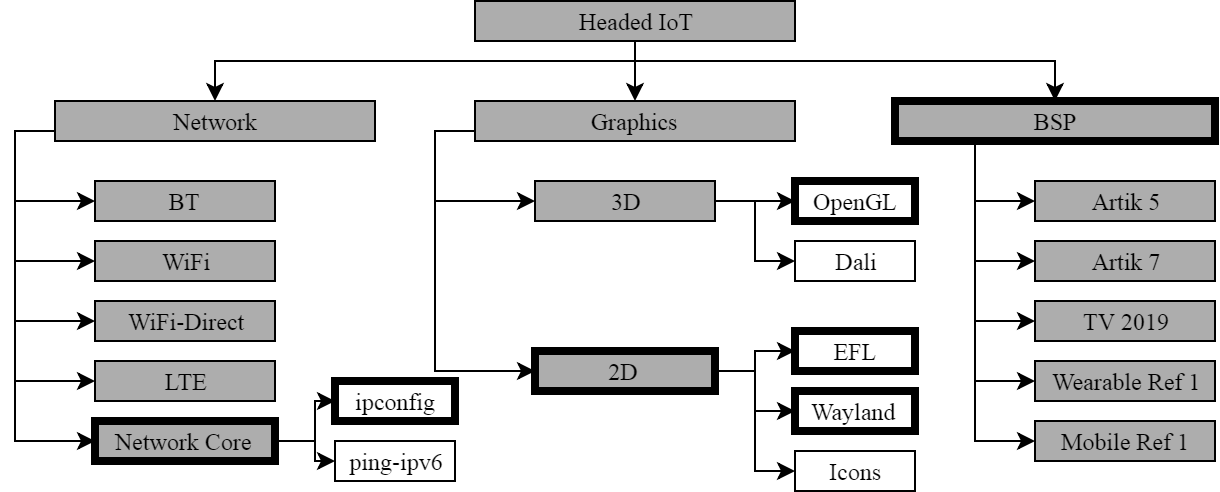
\includegraphics[width=0.95\columnwidth]{figures/BBExample.png}
\caption{Example of building block hierarchy}
\label{FIG_TZN_BBHier}
\end{figure}

Building blocks have the hierarchy between the blocks that can be expressed as a tree with a root node and a leaf node is an individual Tizen package of a empty building block.
Fig.~\ref{FIG_TZN_BBHier} shows an illustrative example of building blocks as a tree.
However, please note that the actual definitions of build blocks are far more complex with a lot of building blocks and individual packages.


In Fig.~\ref{FIG_TZN_BBHier}, boxes filled with gray represent building blocks.
Boxes without gray filling represent individual Tizen packages.
Although most of building blocks are supposed to contain individual Tizen packages, we omitted to simplify the figure.
Boxes with solid thick outlines represent mandatory packages.
Boxes with dashed outlines represent optional packages.
The root node, \texttt{Headed IoT} does not belong to any other building blocks; thus, it is neither mandatory nor optional.


\begin{figure*}
\centering
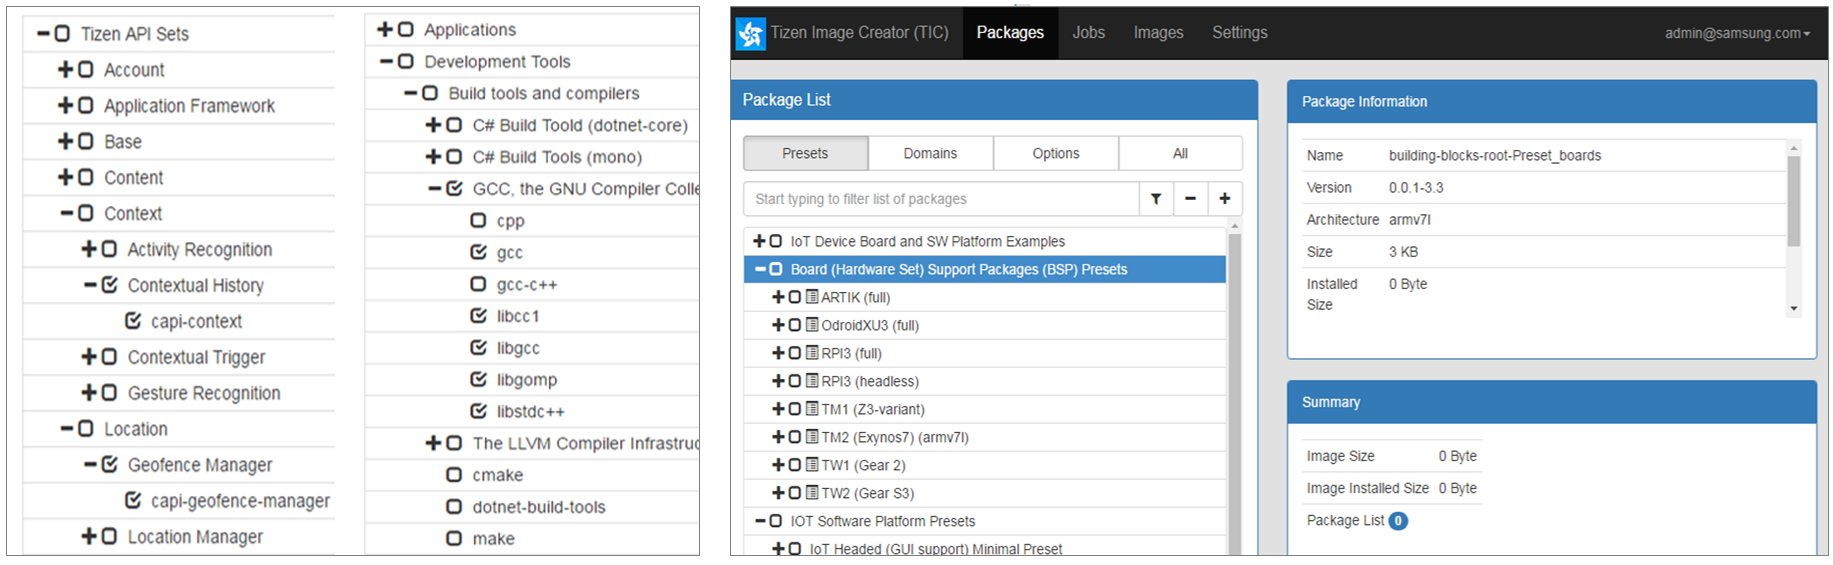
\includegraphics[width=0.96\textwidth]{figures/tic_pkglist_domains_options_presets.png}
\vspace{-0.1cm}
\caption{Building Block hierarchy of May 2017 draft (left) and TIC screenshot where users may choose presets (right)}
\label{FIG_TZN_TIC_SCRSHOT}
\vspace{-0.1cm}
\end{figure*}

%\begin{figure}
%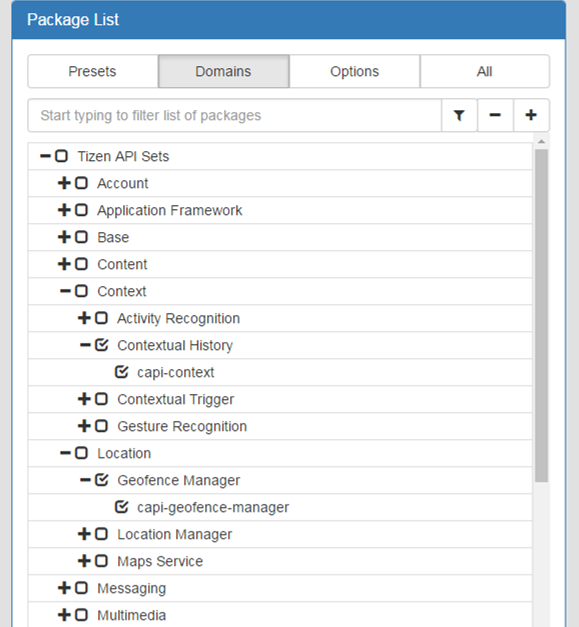
\includegraphics[width=0.47\columnwidth]{figures/tic_pkglist_domains.png}
%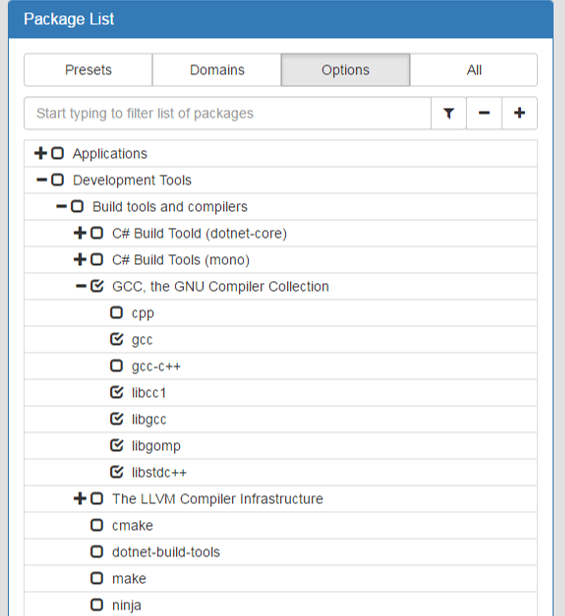
\includegraphics[width=0.47\columnwidth]{figures/tic_pkglist_options_cut.png}
%\caption{Building block hierarchy of May 2017 draft}
%\label{FIG_TZN_TIC_SCRSHOT1}
%\end{figure}

Note that non-hierarchical dependency relations between building blocks are not shown in the figure; e.g., \texttt{TV 2019 Requires 3D}. The hierarchy of building blocks is defined in order to visualize building blocks for users.
The left side of Fig.~\ref{FIG_TZN_TIC_SCRSHOT}, shows how the hierarchy generates building blocks lists for users with TIC, which is to be elaborated in the next section.


In order to make the definitions of building blocks highly readable to project managers and developers and to make the resulting relations consistent, there are a list rules in writing building blocks along with a rule checker that breaks generating building block packages if there is a rule break.
The rule is enforced by a rule checker that is implemented to generate build breaks if there is any violations.
Because the list of rules is too lengthy to be described in this paper, please refer to \cite{7TizenBBRuleURL} for the full list.


%\begin{figure*}
%\centering
%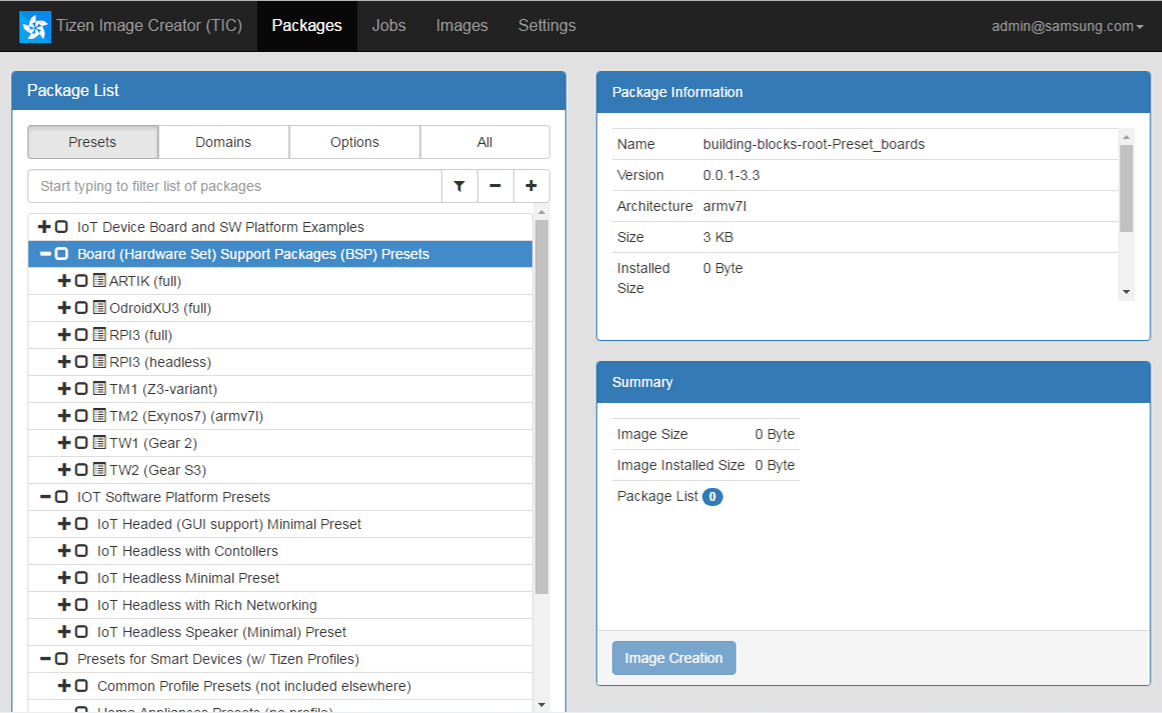
\includegraphics[width=0.80\textwidth]{figures/tic_presets.png}
%\caption{TIC screenshot where users may choose presets}
%\label{FIG_TZN_TIC_SCRSHOT2}
%\end{figure*}

\subsection{Tizen Image Creator (TIC)}\label{SS_TIC}

Tizen experts can prototype software platforms easily with building blocks.
However, third party developers or novice developers require more user-friendly methods than writing a KickStarter~\cite{9TizenKSGitURL} \texttt{.ks} file.
With web application experts, we have developed TIC, which visualizes building blocks and individual packages with their relations and capabilities and configures platforms.


The right-hand side of Fig.~\ref{FIG_TZN_TIC_SCRSHOT} is a screenshot of TIC in a web browser.
There are three categories of building blocks: \texttt{Presets}, \texttt{Domains}, and \texttt{Options}.
\texttt{Presets} provide predefined sets of building blocks and individual packages before actually choosing blocks in Domains or Options.
For example, users may start prototyping a TV platform with a TV Preset, which has all basic features of TV.
In TIC interface, users can review the currently selected blocks and  the currently configured software platform as well.


\texttt{Domains} are building blocks defined by Tizen API sets.
\texttt{Options} are additional blocks that may help development, but are not supposed to be deployed to actual products: e.g., debugging tools, text editors, and profiling tools.


When users have completed configuring the software platform, they may order TIC to create the corresponding OS image file in the server so that they can download the file for deployment a few minutes later.
Users may define additional binary package repositories so that they may add their own custom binaries.
Please refer to the presentations and demonstrations of TDC 2017 for more details of TIC~\cite{2Ham2017TDC}.


\subsection{Craftroom}\label{SS_craftroom}

Based on TIC, the Tizen team has opened a public web service, Craftroom~\cite{5CraftroomURL}, which provides much simplified services of TIC.
With Craftroom, users may generate Tizen IoT software platforms based on the hardware specifications and their own IoT applications developed with Tizen Studio~\cite{23tizenstudio2018} within minutes.

\subsection{Side effects on commercialization}\label{SS_sideeffect_TC}

There has been a major concern from release engineers.
In a commercialization build project of a business division, they build the corresponding packages only.
They do not include packages not intended for their profiles in their own build system, which is a fork of Tizen public.
Thus, if we release Tizen as in the form of Tizen:Unified, they may suffer from longer build latencies due to the inclusion of packages not required by their profiles.


In order to resolve this issue, we have implemented an inter-package dependency analyzer to generate the optimal list of source repositories for a specific software platform configuration.
In order to have a minimal fork for a specific commercialization project, the release engineers may use the tool to minimally choose repositories to be forked.



\section{Evaluations}\label{S_eval}

Both Tizen:Unified and Tizen:Configurability are applied and integrated to Tizen 4.0.
We no longer worry about regressions because the infrastructure is configured to be agnostic to profiles and generates build errors for any violations before accepting changes.
The currently developed version, 5.0, has also adopted this work and is working as expected and releasing and deploying binaries for various device types with the configurability intact.
Note that Craftroom~\cite{5CraftroomURL} provides pretty and easy-to-use UI; however, it is not exposing the full capabilities of configuring a platform.
Craftroom simply provides customized software platform based on the user application provided.

\begin{figure}
\centering
  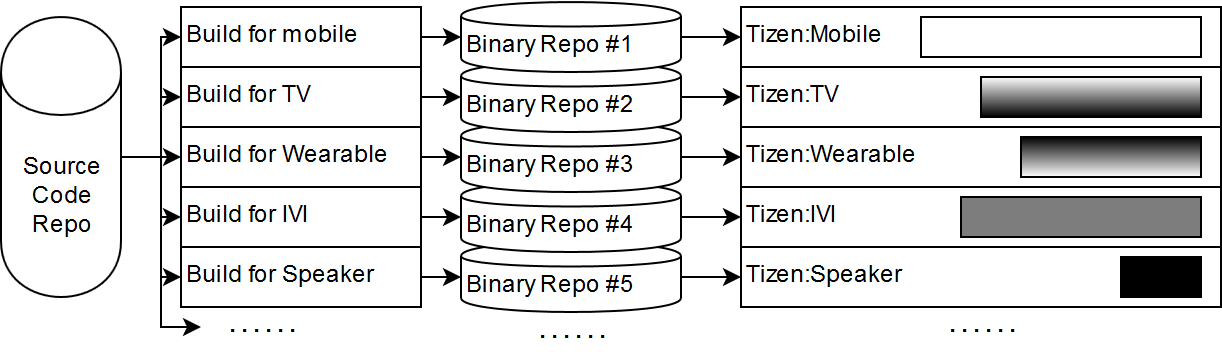
\includegraphics[width=0.95\columnwidth]{figures/TizenInfraBefore.png}
  
  \vspace{0.1cm}
  
  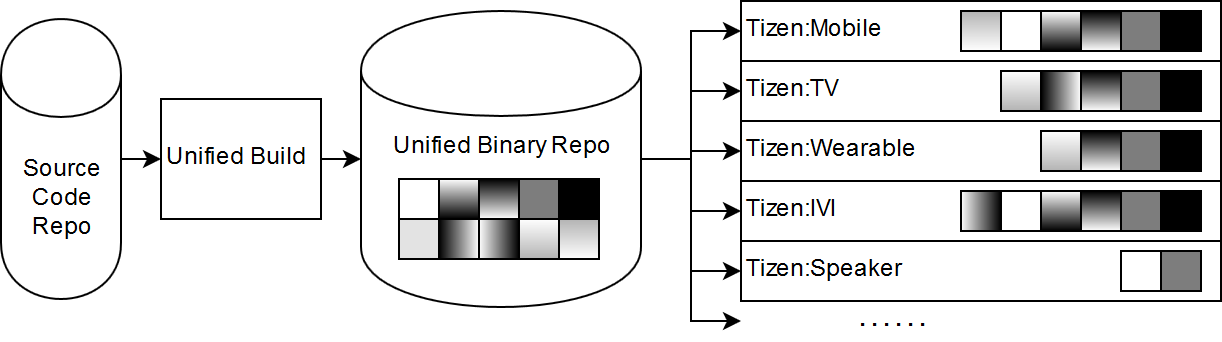
\includegraphics[width=0.95\columnwidth]{figures/TizenInfraAfter.png}
\caption{The infrastructure before and after the work.}
\label{FIG_TZN_BR_INF}
\end{figure}

Fig.~\ref{FIG_TZN_BR_INF} shows how the overall Tizen build, release, and deployment infrastructures before and after this work;
the top shows the infrastructure before this work and the bottom shows that after this work.
Before this work, adding another device type has required to multiply the build workload while it does not after this work.
In other words, adding another device type now only requires to define a new recipe with the given building blocks, which does not increase the workload visibly to the infrastructure or the developers, which requires just a few man-hour for each additional device type.
Note that with the new Tizen prototypes, autonomous driving systems and on-device AI devices, Tizen platform developers have even not been required to know the existence.


\begin{figure}
\centering
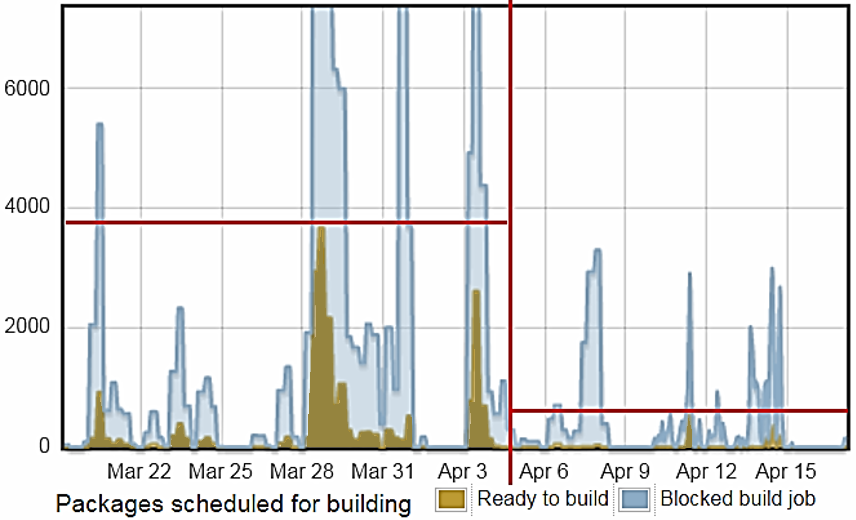
\includegraphics[width=0.95\columnwidth]{figures/tizen_build_obs_buildqueue_4wks_colored.png}
\caption{Build server task queue status in Mar-Apr, 2017}
\label{FIG_OBS_TASKQUEUE}
\end{figure}

Fig. \ref{FIG_OBS_TASKQUEUE} shows the build task workload by describing the waiting task queue lengths.
The dark khaki lines, ``Ready to build``, show the number of packages ready to be built and waiting for resource allocations.
The light blue lines, ``Blocked build job``, show the number of packages to be built, but not ready yet; i.e., even if there are resources available, we cannot build them.
We have migrated to Tizen:Unified from per-profile builds on Apr 4, which is denoted by vertical line in the middle of the figure.
Note that at this stage, Tizen 4.0 had been still in progress and Tizen 3.0 projects (per-profile basis) had been being built as well as Tizen 4.0 projects.


\begin{figure*}
\centering
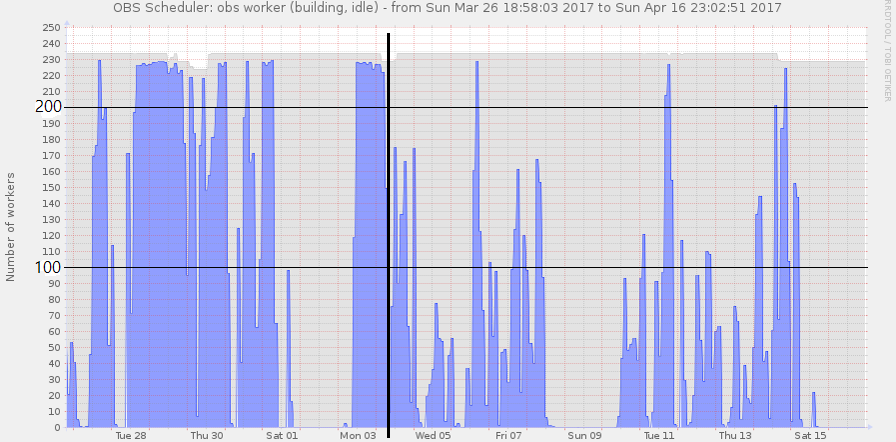
\includegraphics[width=0.90\textwidth,height=5cm]{figures/tizen_build_obs_munin.png}
\caption{Number of busy build servers in Mar-Apr, 2017. Tizen:Unified is applied at the vertical line.}
\label{FIG_OBS_MUNIN}
\end{figure*}

As we can see in Fig.~\ref{FIG_OBS_TASKQUEUE}, the peak queue length has been decreased dramatically from several thousands to less than a thousand.
Normally, the queue length has been reduced to less than dozens or zero from hundreds in typical business hours.


Fig.~\ref{FIG_OBS_MUNIN} shows the number of busy build servers.
We can again see the dramatic reduces of workloads after applying Tizen:Unified to the build system.
After Tizen:Unified is applied, developers usually no longer experience any delays in work queues; in most cases, there have been available build servers waiting for developers! This increases the productivity of developers greatly by allowing developers to get the build and integration results ready for test deployment in shorter time (within an hour, not a day).


With Tizen:Configurability, enabled by Tizen:Unified, Tizen team has started IoT projects (\url{https://wiki.tizen.org/Tizen_IoT}) along with CraftRoom~\cite{5CraftroomURL}.
Further utilizing Tizen:Unified and Tizen:Configurability, a few developers provide continuous integration and deployment services along with software platforms, one for an autonomous driving system and another for on-device AI systems as well, which is named as TAOS.
TAOS is continuously releasing its software platform binaries for both projects with frequent changes in its configurations or creations with new hardware sets and software requirements.


Without the results of Tizen:Configurability, the required build task workload and the complexity of choosing individual packages would have required far more man-month to support the two projects.
We have two members related with TAOS support and most of their workload is due to provide guides to other developers, to implement supplementary developmental tools (profilers and emulators), or to port external software packages for other developers, not on configuring and test-building software platforms.
Note that in the old days, we had needed several experts for such tasks.




\section{Lessons Learned}\label{S_lessons}
In this study, we have observed critical to-dos and not-to-dos. Most of they may seem to be simple rediscoveries of software engineering principles; however, they have been largely ignored in the development process.

\begin{itemize}
\item	Do automate coding rule checks and prevent any mishaps from merging to the source repository. Otherwise, we are destined to lose in the battle against regressions, especially if we have a lot of developers with different backgrounds.
\item	Do not allow code divergences--normally, due to \texttt{\#if} and \texttt{\#ifdef} in C, that results in different binaries per device type. It is a bad technical debt for a software platform.
\item	Do not allow code divergences especially in header files or having different header files per device types. This is even worse; it is contagious to other software packages.
\item	Do promote run-time, boot-time, or install-time device-type discovery; use \texttt{if}, not \texttt{\#if}. Using configuration files (.ini files) parsed in run-time or boot-time is also recommendable.
\item	Do not use any hints of device types or profiles in build configurations or build scripts, except for device drivers, firmware, and kernels. In build-time, the code and its build system should be agnostic to device types or profiles.
\end{itemize}

Fortunately, Tizen is now configured to mandate many of these, relieving us from such concerns.
Commercialization projects usually have forked Tizen itself along with their own build infrastructure in their own company or business divisions, which makes it vulnerable to these concerns.
However, as long as they remain as forked projects, not the mainline projects, any related issues are expected to be cleaned up at every new version releases Tizen; thus, they are ignorable threats for platform developers.



\section{Conclusions}\label{S_conc}

We have unified build projects and binary repositories of the software platform for various device types, improving the developmental efficiency, and proposed the concepts of Building Blocks and the highly configurable platform.
In the due course, we have restructured the Tizen by refactoring hundreds of packages and implementing key infrastructures to support Configurability with Building Blocks.
This work is successfully released via Tizen 4.0 and succeeded to Tizen 5.0 without any developmental overheads to keep the proposed mechanisms intact.


The productivity of both platform developers and infrastructures has improved significantly and Tizen has become capable of providing software platforms for various IoT and edge devices on-the-fly.
The overall productivity of platform developers is improved by reducing turnaround time from code writing to integration and deployment and by reducing the number of binary packages to be created and tested for each source repository.
According to the analysis in May, 2017, by Tizen team~\cite{2Ham2017TDC}, the number of non-base packages built for a full build has been drastically reduced to 968 from 3,483.
Moreover, after the full migration of build systems to Amazon Web Services (AWS), this work saves the cost of running AWS by reducing the number of build tasks.
The improved configurability has allowed creating software platforms for various IoT devices, enabling IoT projects for Tizen and prototypes including autonomous driving systems and on-device artificial intelligence embedded systems.

\section*{Acknowledgements}

We thank our colleagues from Tizen Team and open source communities of Tizen, Red Hat, and openSUSE who provided insight and helped the development.
We especially thank Saikumar Divvela, HyeKyung Kim, and Donghoon Shin for their time and effort for the development, TaeJun Ha, YeongKyoon Lee, and their colleagues for the implementation of the web service, TIC. We also appreciate Gyungpyo Hong, Hong-Seok Kim, Duil Kim, Hyogun Lee, Seunghwan Cho, and Jong-Deok Choi for discussions and support.


% Copy from SBPA2018 Draft
%\begin{abstract}
The wide spread of IoT devices and AI-based edge devices has introduced new challenges for software platforms. In the last decade, the main targets of such platforms, smart phones, wearable devices, and smart TVs, in general and relatively, have well-defined common features and requirements for each of the few device types. However, IoT devices have much longer tails, which make it intractable to define a common software platform profile. With such higher diversities, we can no longer afford individual build configurations per device type, which unacceptably multiplies burdens of developers as well as build systems. Besides, on-the-fly prototyping and creating platforms for new devices is required by both third party and in-house IoT developers. With traditional platform tools, the capability to do so is limited; such tasks usually require rare release and build experts and too much time and effort. With the projects described in this paper, we have successfully addressed the issues: a) unifying Tizen software platform code and its infrastructure to increase the development productivity for multiple device types and b) making Tizen configurable so that even third party developers may create their own Tizen variations on-the-fly easily and quickly. This has enabled a public service, CraftRoom.tizen.org, where IoT developers may acquire their own customized Tizen on-the-fly for their own products. This work is integrated into Tizen 4.0 and later as open source software. Based on this work, Tizen team has started IoT platforms and we have adapted Tizen to autonomous vehicle systems and AI software platform with affordable costs.
\end{abstract}

\section{Introduction}
Traditionally, software platforms for smart devices (e.g., Tizen, Android, and iOS) have clear target device profiles—phones, wearables, tablets, or TVs—, which define mostly (if not completely) common API sets, features, and requirements across different hardware sets. However, the wide spread of IoT devices has introduced the new challenge: the long tail of the IoT [1]. The long tail of the IoT incurs the following significant challenges for software platforms:
\begin{itemize}
\item Each IoT device and application might require their own customized software platform: Configurability.
\item With various device types, various OS images are to be built from the same source codes with different configurations. Then, we need to build and unit-test too many times. Build systems are required to do the same as well: Build Explosion.
\end{itemize}

Both challenges have induced significant but affordable costs with traditional smart devices. However, with the long tail of the IoT, this is no more affordable. Even if we have only 10 different IoT devices, not 100, developers need to build 10 times for each commit and the build system gets additional x 10 workloads. This is especially unacceptable with the long tail-ness; each IoT device type is going to have little revenue although the whole IoT device portfolio may have a lot. We cannot afford linearly increasing platform development costs with the increasing number of IoT device types. Tizen platform developers had been already overloaded with repeated build and test workloads per profile and overly waiting for overloaded build systems. Thousands of build and test tasks had to wait several hours in a queue during busy hours even though we had more than 200 powerful build servers.


Before addressing Configurability, we have addressed Build Explosion first because we should be able to build software packages for various devices types without causing additional workload for both platform developers and build systems. We have addressed Build Explosion by unifying the Tizen build procedures and binary repositories, enforcing every profile to share the same set of binary packages, not only the source codes; a.k.a., Tizen:Unified project.


In order to unify Tizen, we have introduced new rules for platform developers and plugin architectures with new binary dependency rules, enforced by build systems and Linux packaging systems, which are upstreamed to the open source communities as well so that the new rules becomes the standard. Thanks to the cooperation from platform developers and the communities, we could unify Tizen binaries into one build project and prevent any further diverges from the unification since Tizen 4.0 in 2017.


Unifying binary repositories of Tizen has mitigated the build workload of not only for new IoT devices, but also for the traditional smart devices. Tizen project (Tizen:Unified in \url{https://build.tizen.org}) no longer builds five times for five profiles, but builds only once for all. After the migration to Tizen:Unified, peak build task waiting queue size has dropped from thousands to tens [2].


With Tizen:Unified completion, we could apply the infrastructure designed to support Configurability with Building Blocks to Tizen. Based on Tizen:Unified, building block definitions [3][4] provide easy-to-configure components to build a custom software platform. Note that although first building block definitions were written by authors, the current “release” definitions are written by Tizen team. Tizen Image Creator (TIC) [2] offers a web user interface to configure a custom software platform even easier. Based on TIC, Tizen offers an instant software platform creation service for IoT developers, Craftroom [5]. TIC and Craftroom provide a customized software platform for IoT developers within minutes, not hours or days.


\begin{figure}
\label{FIG_TZN_BR_INF}
\missingfigure[figwidth=6cm]{FIG 1 in SBPA18}
\caption{Tizen build and release infrastructure. Before (top) and after this work (bottom).}
\end{figure}

Fig. \ref{FIG_TZN_BR_INF} shows how the overall Tizen infrastructure has been improved with this work. Based on this work, we are also delivering customized software platforms (OS and development environments) for autonomous driving systems and STAR on-device platform in AI Center as well.
By unifying Tizen and providing configurability with building blocks, we have reduced build and test workloads significantly and enabled Tizen for wider ranges of device types with significantly reduced workloads.







\section{Contributions}

We have constructed both projects, Tizen:Unified and Tizen:Configurability, refactored Tizen platform software packages, restructured build procedures and rules, which enabled on-the-fly platform customizations. Build and packaging rules introduced in this work are either within the Linux standard (Redhat/OpenSUSE) or upstreamed to the community as a new standard. 


This work is applied to Tizen 4.0 (2017) and 5.0 (2018), enabling various new products and prototypes, ranging from home appliances and various IoT prototypes to autonomous driving systems and AI on-device platforms. The Tizen:Unified/Configurable team has been relatively small and consisted of four members, which indirectly shows the efficiency of the project as well. The four members have had the following roles.


One member, a server script writer, has implemented various tools for other members, including regression detector, overall Tizen source code quality monitoring tools, and test build server utilities. Another member, while refactoring a few packages, has focused on communicating developers and reviewers, persuading, negotiating, or reminding them to improve or accept our refactoring patches. The other two members have focused on refactoring hundreds of packages.


There had been a few packages that could not be entirely refactored by this team. Such packages are either too huge or have complicated dependencies with other packages: EFL, input subsystems, and web browser. For such packages, we have extensively guided and cooperated with the corresponding developers. In the earlier phase of the project, we have held several seminars and meetings for the entire Tizen developers or lead developers to let them understand what was going on and why we were doing it.


\section{Related Work}

\subsection{Linux binary package management}

Mancinelli et al. [11] contribute an effective and automatic way to support distribution editors in handling those issues that were, until now, mostly addressed using ad-hoc tools and manual techniques. Most of  the existing approaches on the problem of managing dependencies are targeted at designing component systems, with a clear top-down process typical of a software architecture viewpoint, while the component systems we have to handle come from the huge preexisting infrastructures. They described their framework they have developed for managing the complexity and improving the quality of large package based Free and Open Source Software (FOSS) systems. Their tools were used at Caixa Magica and Mandriva distribution in parallel with their standard distribution life cycle phases.


Software Build Systems [12] describes an extensive treatment of the software build process including the choices, benefits, and challenges of a well-designed build process. It surveys the tools and techniques for building software products and the ways things go wrong. It depicts that inadequate build systems can dramatically impact developer productivity. For example, bad dependencies, false compile errors, failed software images, slow compilation, and time-wasting manual processes are just some of the byproducts of a subpar build system. Also, he explains how to optimize the performance and scalability of your build system. 


Galindo et al. [13] address the issues such as the lack of realistic variability models to evaluate those techniques and tools is recognized as a major problem by the community. They suggest that Debian packages dependency language can be considered as a variability language. Also, they provide a mapping from this language to propositional formulas enabling their analysis by means of SAT solvers. They focus on other variability dependency language existing in open source community increasing even more the availability of realistic variability models up to 20,000 packages to the Software Product Line (SPL) community. However, they do not detect anomalies in Debian models such as conditionally dead packages or redundancies.


Cosmo et al. [14] point out why the upgrade problems faced by Free and Open Source Software distributions have characteristics not easily found elsewhere. While for detectable failures trade-offs can be made using snapshot and appropriate partitioning, no fully generic solution exists to counter upgrade failures. They survey current countermeasures to such upgrade failures, argue that they are not satisfactory, and sketch alternative solutions. They only concentrated on applying fingerprinting techniques to cluster maintainer scripts of Debian distribution to get a clear view of all their use cases.


Adoption of Academic Tools [15] presents an overview of 10 years of research in this field and the process leading to the adoption of our tools in a FOSS community. They presented three tools such as distcheck and buildcheck, which scan all the packages in a Debian distribution to identify installability issues. They focused on the Debian distribution and in particular they looked at the issues arising during the distribution lifecycle: ensuring buildability of source packages, detecting packages that cannot be installed and bootstrapping the distribution on a new architecture. 


Schroeder [16] depicts the package dependency solver library that is called SAT solver. This project was started in May 2007 when the zypp folks decided to switch to a database to speed up installation. It also offers an efficient file and memory representation for the usually complex repository and dependency data, with attributes support. The SAT solver of Libzypper is a port from the red carpet solver, which was written to update packages in an already installed system. Using it for the complete installation progress brought it to its limits. Also, the added extensions support an audit functions for weak dependencies and patches made it fragile and unpredictable. 


\subsection{Build systems}

GBS (git-build-system) [17] is a developer command line tool that supports Tizen package development. It is used to generate tarballs based on Git repositories, to do local test buildings, and to submit code to a main build service of Tizen, OBS. From the package maintenance point of view, GBS divides packages into these two categories: native packages where Tizen is the upstream and controls the source code repository and non-native (or upstreaem) packages for which Tizen is not the upstream such as the Linux kernel or zlib.  GBS determines a package as non-native, if the git repository has an upstream branch. The actual name of the upstream branch can be configured using the 'upstream\_branch' in option in the .gbs.conf file. GBS supports manually maintaining patches, that is, outside the automatic patch generation. This may be needed for architecture-dependent patches, for example, as GBS patch generation does not yet support conditional patches. 


MIC (Mobile Image Creator) [18] is to create images for Tizen software platform.  With the MIC tool, users can create images of different types for different verticals, including live CD images, live USB images, raw images for KVM, [21] loop images for IVI platforms, and filesystem images for chrooting.  Also, users can chroot into an image using enhanced chroot command of MIC. Besides, it enables converting an image to another image format, a very useful function for those sensitive to image format. 


Open Build Service (OBS) [19] is a general build, release, and package-distribute system for various target platforms in an automatic, consistent and reproducible way. OBS enables to release software for a wide range of operating systems and hardware architectures. It is an open and complete distribution development platform that provides a transparent infrastructure for development of Linux distributions, used by openSUSE, Tizen and other distributions. Also, it supports Fedora, Debian, Ubuntu, RedHat and other Linux distributions. Also, it provides extensible web interfaces and APIs. The build process executes all the instructions that it finds in the build recipe. If the build is successful, the files of the package are installed into a sandbox, where the binary packages are created; the packages are released as RPM [23] by default. Then, the packages are released and deployed via repository compatible with package managers.


Zypper [20] is a package manager that installs, updates, and removes packages and manages repositories. It is especially useful for managing software packages remotely or with shell scripts. With zypper, we can easily update the distribution. Besides, we can update the software platform in run-time. Note that Tizen is fully compatible with zypper although it is not included in most traditional Tizen profiles.


\section{Design and Implementation}

This chapter elaborates the design of Tizen:Unified and Tizen:Configurability projects and how we have implemented and progressed with the projects.

\subsection{Issues of Tizen before 4.0}

The Pre-4.0 Tizen had a single build project for each profile: i.e., mobile, wearable, TV, IVI, and common. Note that “common” profile does not stand for a common part of other four profiles. It had been simply yet another profile that had an ambiguous device type; often it had been considered to be the superset of other profiles as well.


With such concepts of profiles, creating a new device type, which happens very frequently with IoT devices, requires to define a new Tizen profile and build project. Then, it incurs redundant build workloads increasing proportionally with the number of profiles. Even if the source code is the exactly same, we are forced to build the whole Tizen repeatedly, which is already too expensive with five profiles.


If we need to do prototyping with device types or software platforms, juggling with the configuration of OS images, such overheads makes it almost impossible; the administrators of build system servers will not allow you to create and keep modifying Tizen profiles in the build servers already overloaded, where developers and managers keep complaining about the build latencies.


Even if we may prototype new Tizen profiles, having extremely vast number of powerful servers, prototyping new profiles is too difficult for non-build-expert developers. To configure a new profile, we need to fully understand the Tizen meta-packages and the underlying mechanisms of build and imaging systems. Even in the Tizen platform team, there are less than a dozen people with such capabilities.


\subsection{Achieving build unification}\label{S_ach_build_unif}

We have achieved the unification of Tizen builds for Tizen 4.0 by April, 2017. By unifying the Tizen builds, we could remove profile specific builds—such as “Tizen:Mobile” or “Tizen:TV”—and provide a single build operations and their results for all Tizen profiles with the name of  “Tizen:Unified”.


The objectives of Tizen build unification includes: a) shorter build latencies by eliminating duplicated builds of a software package to make it affordable to support many different profiles, b) allowing to create arbitrary profiles from a single shared binary repository, and as a results of a) and b), c) allowing to create new profiles on-the-fly without rebuilding software packages, enabling the next big step, “Configurable Tizen”.


There are two major rules to achieve the unification of Tizen builds:

\begin{itemize}
\item In build-time, build processes (build scripts, compilers, and build systems including OBS [19] and GBS [17]) should not be able to identify the target profile or device except for the architecture: e.g., armv7l and x86\_64. However, processes may identify the profile or device type at install-time and run-time.
\item Every single binary package (RPM [23] package) of Tizen should be able to co-exist in a single repository as long as the package has the same target architecture.
\end{itemize}

With the completion of the unification, these rules are applied for all Tizen packages and have been kept so far. With the completion, the build system is configured to enforce the rules automatically so that any violating changes cannot affect the system since Tizen 4.0 [2].


The most significantly challenging issue has been the huge number of Tizen software packages. Tizen:Common had 822 packages in April, 2017 [2]. When we started planning Tizen:Unified project in July, 2016, we had 134 packages to be refactored to satisfy the rules. When we started refactoring with the relatively small team members of four in November, 2016, the number of refactoring target packages has increased to 171.


Another significantly challenging issue for the unification is the regression, where a complying package is modified to violate the rules. We had multiple cases where packages refactored to comply being modified to violate by developers. We have also observed multiple packaging complying from the beginning become violating suddenly during the project, increasing the number of refactoring targets further.


Ideally, the refactoring of each and every package is better executed by the main contributor or maintainer of the package. However, it requires each and every main contributor and maintainer to fully understand the rules, the mechanisms of build systems, and how to refactor their own packages for Tizen:Unified with their own feature and bugfix workload. During the early phase of Tizen:Unified project, as a pilot program between July 2017 and August 2017, we have tried the “ideal” method with few small groups along with full assistance from the Tizen:Unified team. As the result of the pilot program, we have learned that the following points:


\begin{itemize}
\item We should not expect that each main contributor to understand the underlying build system of Tizen. They are users, not developers of the build system and a good build system does not require its users to understand the build system itself.
\item It is extremely difficult to ensure that the rules are kept during active software development where new commits are applied daily if not hourly.
\item Applying yet another coding rule requires additional burden to developers. Even if we could have justified the need to a few key members (small team leaders and main contributors), it was often not enough to let them put some additional efforts to prevent others from breaking the rules or review more carefully. Moreover, we could not enforce the rules with build systems until each and every package follows the rule perfectly; otherwise, we will get build breaks with every snapshot and the whole Tizen team will not be able to function properly.
\end{itemize}


As a conclusion from the points, we have decided to do all the refactoring and find how to refactor for each package in Tizen. However, a few packages (Chromium, EFL, and local/input systems) had much complicated issues that enforced us to rely on their own main contributors to refactor the packages.


During the progress of Tizen:Unified project, to detect any attempts of regression, we have developed and operated a gerrit [6] monitoring service that reviews incoming commits and find any possible regressions from them. In many cases, we could have prevented such commits being merged in time.


During the project, we have categorized to-be-refactored packages into the following types:
\begin{enumerate}[A.]
\item The build script is aware of the profile. It may use different source code per the profile (“%profile” macro defined by the build project). Often the source code has compiler preprocessor conditional statements (#ifdef) activated by the build scripts.
\item Multiple git repositories generate packages with a common name. For example, both mobile/…/efl-config.git and wearable/…/efl-config.git had generated efl-config.
\item The build script depends on a package, model-build-features. The package, model-build-features, generates macro definitions based on the profile or device types, affecting build scripts of other packages.
\end{enumerate}

We have observed a lot of useless dependencies on the profiles or device types and removed them immediately. We also have had cases where the dependencies are easily removed by using configuration files in /etc. 


\subsubsection{Runtime profile identification}\label{SS_RUntimeProfileId}

If we cannot avoid per-profile behaviors of a package, applying the runtime profile identification mechanism is recommended. This mechanism is recommended because it allows having a fully unified binary for the package across different profiles without the need for installing different binary packages for each profile. The only more recommendable method is to behave exactly same regardless of the profile definition itself, which is sometimes impossible. Many Type-A cases have been resolved by this.


In order to allow runtime identification, we have used a Tizen API to detect the profile and removed all preprocessor conditionals related. Many of such refactoring commits can be found with the URL: \url{https://review.tizen.org/gerrit/#/q/message:%22remove+profile+build%22+status:merged+message:%22runtime%22} (you need to login to review.tizen.org with Tizen.org accounts before entering the URL.)


Table \ref{TABLE_CODE_IFDEF} shows a simple example where such refactoring is beneficial and Table \ref{TABLE_CODE_IF} shows the refactored code. 

%% TODO : Check the template if this is allowed.
\begin{table}
\begin{verbatim}
#ifdef PROFILE_MOBILE
Do_mobile_action();
#else
Do_common_action();
#endif
\end{verbatim}
\label{TABLE_CODE_IFDEF}
\caption{Type-A per-profile code with \#ifdef}
\end{table}

\begin{table}
\begin{verbatim}
if (get_profile() == PROFILE_MOBILE)
    Do_mobile_action();
else
    Do_common_action();
\end{verbatim}
\label{TABLE_CODE_IF}
\caption{Refactored code}
\end{table}

\subsubsection{Inter-package dependency management}

Sometimes, we have created different binary packages for each profile or device types along with meta packages or virtual packages (RPM [23] capabilities) to make per-profile differences transparent to other packages.


Let us assume that we have a package X, which needs to have different contents for its binaries for mobile profile. Then, we can modify the build scripts of RPM (.spec files) to generate “X-profile\_mobile.rpm”. The first variation of the mechanism is to generate “X.rpm” file for other profiles and to generate “X-profile\_mobile.rpm” to declare that it may act as “X.rpm” by adding inverse-dependency of “Provides: X”. The second variation is to create a meta package, “X.rpm”, without any files, but with meta data only stating that it has dependencies on its subpackages or plugins, “X-compat” and to create plugin subpackages of mobile and other profiles declaring that they provide “X-compat”, which enforces to install one of such plugins to install “X.rpm”.


Note that for the first variable, “X.rpm” needs to declare that it provides “X-profile\_common”, “X-profile\_wearable”, and so on in order to be explicit for per-profile configurations. Besides, both variations require plugins to declare “Conflict” statements to prevent installing plugins of different profiles for one main package. The first variation is usually applied when only few profiles require different binaries. The second is usually applied if each profile has its own plugins or configuration files.


The example of the first variation is the commit 4fad77614 of libsvi (\url{https://git.tizen.org/cgit/platform/core/system/libsvi/commit/?id=4fad77614ae6916670b22a1e8dac0d49e87a5d4b}). The example of the second variation is the commit 53135dcb of model-config-baytrail (\url{https://git.tizen.org/cgit/platform/adaptation/intel_baytrail/model-config-baytrail/commit/?h=tizen&id=53135dcb7ed8f2d332f7437de08d5b0aa4332179}).


A critical side effect of this mechanism is that the Tizen build system (both OBS [19] and GBS [17]) gets confused by multiple candidates for inter-package dependency resolutions if a package depending on the package with this mechanism applied is being built. In other words, if X.rpm is required by Y.rpm when we build Y.rpm, the build system cannot determine whether it should install X-profile\_mobile.rpm or the other; both are allowed and build systems are not allowed to accept such ambiguity.


We can resolve such ambiguity by adding weak dependencies, Recommends. The contents of binaries do not matter for build dependents if they are shared objects; only their forms (header files) matter, which holds for Tizen native platform binaries. However, we had exceptions to this, mentioned in the next section; the contents of external headers (APIs) differ per profile.



\begin{figure}
\label{FIG_TZN_TYPEB_RESOL}
\missingfigure[figwidth=6cm]{FIG 1 in SBPA18}
\caption{The left shows the first variation and the right shows the second variation}
\end{figure}

Fig. \ref{FIG_TZN_TYPEB_RESOL} elaborates inter-package dependency management mechanism. Note that any packages external to X should not explicitly depend on profile plugin subpackages (*-profile\_*.rpm). Such packages should refer to the main package (X in Fig. \ref{FIG_TZN_TYPEB_RESOL}) only and let the package management system handle the rest.


Type-B and Type-C are mostly resolved by declaring inter-package dependencies explicitly after properly refactoring the build scripts and source codes so that per-profile parts are separated into different binary packages. There are many Type-A cases resolved by this mechanism as well when it is too difficult to apply the mechanism of the Section \ref{SS_RUntimeProfileId}. It is usually when a profile has completely different source code files, which incurs too large modifications to apply runtime profile identifications. In such cases of Type-A, we generated different executables for each profile and packaged them into different binary packages, which is often referred as sub packages. However, for the package management mechanism, there are no differences between packages and sub packages.


\subsubsection{Inappropriate definitions of APIs}

Unfortunately, Tizen developers have generated external header files with different function declarations per profile or even different header files are used per profile. Moreover, there had been an extreme case where Tizen public API header has different C enum definitions per profile: https://git.tizen.org/cgit/platform/core/api/player/commit/?id=006bfe52966343e974f665f2ea85f05ec62de45e. In this case, the C enum definitions of mobile had been PLAYER\_DISPLAY\_TYPE\_EVAS = 1 and PLAYER\_DISPLAY\_TYPE\_NONE = 2 while those of wearable had been PLAYER\_DISPLAY\_TYPE\_EVAS = 2 and PLAYER\_DISPLAY\_TYPE\_NONE = 1. This extreme case has required Tizen public API changes that may make previous applications incompatible with new Tizen versions. Thus, as in the commit mentioned above, we redefined C enum values and defined old values (1 and 2) as obsolete along with compatibility resolving code that behaves differently for each profile.


For the first case, where different function declarations are used per profile by using compiler preprocessor conditionals, we have manually refactored header files removing all preprocessor conditionals. We cannot apply the mechanism of Section 4.2.2. for headers exposed externally because the depending package (“Y.rpm” in the examples of Section 4.2.2.) cannot be identical for different profiles; profile dependency is no more transparent to external packages! \url{https://review.tizen.org/gerrit/#/c/96504/} is an example of this case. \url{https://review.tizen.org/gerrit/#/c/96504/} is an example of this case. 


The resolution for the second case is same as the first case. It requires manual inspection and refactoring as well, but with more care and efforts as the difference is larger. A fortunate case (where only the comments differ) is \url{https://review.tizen.org/gerrit/#/c/101404/} while an unfortunate case is \url{https://review.tizen.org/gerrit/#/c/96504/}.


\subsubsection{Workarounds}

There are a few cases where we cannot completely remove the dependencies on profiles or device types from the binary packages except for the plugin subpackages, which do not incur external dependencies.

\begin{enumerate}
\item Device drivers or kernel binaries require dependencies on device types and often, such dependencies are hardcoded.
\item We are not allowed to generalize product or business division specific routines. A business division has required keeping their product specific conditional codes embedded in Tizen while such codes cannot be generally used for other profiles or devices. Although, in principle, this is undesirable as it fragments the source code and damages the readability because it usually heavily depends on preprocessor macros, this has been something we could not alter.
\end{enumerate}
Case 1 includes Linux kernel, which is built and installed for all devices, but their source code repositories or build configuration might differ. We have applied an altered method of Section 4.2.2 as shown in Fig. \ref{FIG_TZN_KERNELDEP}.


\begin{figure}
\label{FIG_TZN_KERNELDEP}
\missingfigure[figwidth=6cm]{FIG 1 in SBPA18}
\caption{The altered method of Fig. \ref{FIG_TZN_TYPEB_RESOL} for Linux kernel}
\end{figure}

As shown in Fig. \ref{FIG_TZN_KERNELDEP}, different Linux kernel binaries from various git source repositories provide the capability of “Linux-kernel” so that any package or software platform manifests requiring “Linux-kernel” can be satisfied with one of Linux-kernel binary packages. However, as mentioned before, we cannot have multiple candidates for a single dependency (or capability in RPM documents) in build time. Thus, for external kernel module repositories, a representative kernel repository has been chosen to provide the “Linux-kernel-modulebuild” capability, which is the emulator kernel repository. Note that we can have a single representative for each Linux kernel version. Therefore, if there are multiple Linux kernel versions required for a specific Tizen version, we can choose multiple representatives, one for each kernel version. We may choose multiple representatives without introducing the ambiguity for build systems by specifying kernel versions in kernel modulebuild dependencies. That is “BuildRequires: linux-kernel-modulebuild = 4.4.0” and “Provides: linux-kernel-modulebuild = 4.4.0” instead of “BuildRequires: linux-kernel-moduilebuild” and “Provides: linux-kernel-modulebuild”.


For case 2, we have configured the Tizen main public build systems to ignore any macros related with products or business divisions. Although we have allowed preprocessor macro conditionals for products and business divisions, as long as the main build system ignores such macros, we can guarantee that the resulting binaries are complying Tizen:Unified. Simultaneously, with the same source code repositories, a business division may keep their own special source code activated in their own build projects in their own private build systems. However, codes creating different binaries under the same package names should be discouraged. Such codes are usually the results of laziness (or overloaded workloads) of developers; they should have used configuration files (.ini files in /etc directory) or accessed Tizen device APIs, probing device type, name, and profiles. We hope, in some day, such lame codes are totally eliminated.


\subsubsection{How we have progressed}

Regressions by incoming new commits breaking the rules mentioned in Section \ref{S_ach_build_unif} have been headaches for the Tizen:Unified team members. Before April, 2017, during the active development of Tizen:Unified project, the build system could not be configured to ignore per-profile build configurations. Thus, we have constantly reviewed incoming Tizen commits with a monitoring service we have implemented to find any regressions. Such regressions are notified to our team, which, in turn, allow us intervene the related activities. In most cases, we could have successfully dropped or corrected such commits before merging.


Once every single package in Tizen has obeyed the given rules to keep Tizen unified, we have removed all per-profile build projects from the build system and unified all Tizen packages into a single build project named “Tizen:Unified”, which does not allow any dependencies on profile or device types in building Tizen packages. Note that build projects for older versions (e.g., Tizen 2.x or 3.0) are untouched and kept with per-profile basis; however, they are no more actively developed and do not require heavy build workloads as currently developed versions. Another build project, “Tizen:Base” exists independently in order to reduce the performance impact from cyclic build dependencies of toolchains. Cyclic build dependencies incur heavy redundant build workloads and are prohibited in Tizen:Unified because it is expected to be rebuilt frequently; most developers contributes to Tizen:Unified daily. Note that as long as multiple build projects do not share the same source repository and inter-project dependency is acyclic, there is no build performance problem and on-the-fly configurability.


We can add a disjoint build project that does not have cyclic inter-project dependencies without any deterioration on the performance or the configurability. Thus, we can create many prototypes aggressively and quickly. In the autonomous driving project and the on-device AI platform project, we have a lot of additional source repositories, over 100. As long as these two projects are not officially accepted as Tizen public—we are prototyping!—, it is not allowed to add such packages (over 100) to Tizen:Unified build project.


By adding a disjoint build project, depending on Tizen:Unified, Tizen:TAOS (representing Tizen AI OS Support, Tizen Autonomous-driving OS, and Tensor-Aware OS simultaneously), we are aggressively prototyping new software platforms for these two new projects. When there is a new need for yet another variation, a single developer can generate and deploy a new software platform and its binary images to corresponding developers and devices within few hours, which is frequently occurring. The inter-project dependencies are shown in Fig. \ref{FIG_TZN_INTERPDEP}.

\begin{figure}
\label{FIG_TZN_INTERPDEP}
\missingfigure[figwidth=6cm]{FIG 1 in SBPA18}
\caption{Inter-project dependencies of Tizen build projects. The top shows pre-4.0 and the bottom shows 4.0 or later.}
\end{figure}

\subsection{Achieving configurability}

With the completion of Tizen:Unified project, Tizen has achieved the basic ability to configure a software platform on-the-fly. Because every single binary package can be located in a single package repository and there is no more ambiguities between package names any more, we can now use package management systems without glitches anymore: zypper, DNF, or yum, which are equivalent to apt in Ubuntu/Debian systems.


For most workstations, PCs, or servers, this degree of configurability is enough and we may have nothing more to progress. However, it does not hold for embedded systems or a deployable device set consisting of both devices and software platform. For such systems, we need to continuously release and deploy OS images that can be flashed to devices easily without much manual labor. Traditionally, in Tizen, we have been using a tool named MIC; MeeGo Image Creator, renamed as MIC Image Creator after the demise of MeeGo project.


Issues with traditional MIC and its supporting tools are:

\begin{enumerate}
\item It is too difficult to create a new software platform configuration (.ks file) for most users; you need build system experts who understand Tizen and its infrastructure deeply. Thus, it can be practically impossible for most third party developers to create Tizen prototypes.
\item You need your own dedicated Linux workstation to create Tizen images. It would be more appropriate if IoT application developers with an access to web browsers and Tizen Studio [23] can write their own IoT applications and generate proper Tizen OS images for their own IoT devices and applications on the fly.
\end{enumerate}

In order to address Issue 1, we have introduced the concept of building blocks and implemented the first draft in \url{https://git.tizen.org/cgit/tools/building-blocks/} in May, 2017. The concept of building blocks is now the core of Tizen profiles and device type definitions. It is also the main tool for project managers. With building blocks, users can create prototypes without the knowledge of thousands of individual Tizen packages or to choose hundreds from them, but with the fewer (about one or two dozens) abstract and easy-to-understand building block names: e.g., Bluetooth, Haptic, and Default-App-Setting.


In order to address Issue 2, we have introduced Tizen Image Creator (TIC), which has the web frontend with node.js. Analyzing individual packages and generating deployable OS images for the configured prototype is executed in a web server. However, the service and the code of TIC is not opened to the public. The code of TIC is opened to Samsung internally only in the Samsung gerrit server: \url{http://suprem.sec.samsung.net/gerrit/}.


There is publically opened web service that has TIC as its backend at \url{https://craftroom.tizen.org}: Craftroom. Craftroom service offers much simplified and easier interfaces specifically focused on IoT developers. Note that Craftroom itself is designed and developed by another team along with a UI/UX team; we have provided its backend (TIC) and enabling infrastructure (Building Blocks).


\subsubsection{Building blocks}

A building block is a meta packages that designates mandatory packages and optional packages. As a meta package, it does not have its own files, but has dependency relation information consisting the list of mandatory or optional packages. A mandatory package is an individual Tizen package or another build block that is installed if the corresponding building block is chosen. An optional package is an individual Tizen package or another building block to be shown in the user interface if the corresponding building block is chosen. Unlike mandatory packages, optional packages are not automatically chosen with the corresponding building block.


\begin{figure}
\label{FIG_TZN_BBHier}
\missingfigure[figwidth=6cm]{FIG 1 in SBPA18}
\caption{Example of building block hierarchy}
\end{figure}

Building blocks have the hierarchy between the blocks that can be expressed as a tree with a root node and a leaf node is an individual Tizen package of a empty building block. Fig.5. shows an illustrative example of building blocks as a tree. However, please note that the actual definitions of build blocks are far more complex with a lot of building blocks and individual packages.


In Fig. \ref{FIG_TZN_BBHier}, boxes filled with gray represent building blocks. Boxes without gray filling represent individual Tizen packages. Although most of building blocks are supposed to contain individual Tizen packages, we omitted to simplify the figure. Boxes with solid thick outlines represent mandatory packages. Boxes with dashed outlines represent optional packages. The root node, “Headed IoT”, does not belong to any other building blocks; thus, it is neither mandatory nor optional. 



\begin{figure}
\label{FIG_TZN_TIC_SCRSHOT1}
\missingfigure[figwidth=6cm]{FIG 1 in SBPA18}
\caption{Building block hierarchy of May 2017 draft}
\end{figure}

Note that non-hierarchical relations between building blocks are not shown in the figure; e.g., “BT” requires “WiFi”. The hierarchy of building blocks is defined in order to visualize building blocks for users. Fig. \ref{FIG_TZN_TIC_SCRSHOT1}, shows how the hierarchy generates building blocks lists for users with TIC, which is to be elaborated in the next section. 


In order to make the definitions of building blocks highly readable to project managers and developers and to make the resulting relations consistent, there are a list rules in writing building blocks along with a rule checker that breaks generating building block packages if there is a rule break. The rule is defined as human-readable text in [7] and the rule checker is defined in [8]. Because the list of rules is too lengthy to be described in this paper, please refer to [7].


\begin{figure}
\label{FIG_TZN_TIC_SCRSHOT2}
\missingfigure[figwidth=6cm]{FIG 1 in SBPA18}
\caption{TIC screenshot where users may choose presets}
\end{figure}

\subsubsection{Tizen Image Creator (TIC)}

Tizen experts can prototype software platforms easily and quickly with building blocks. However, third party developers or casual developers require approaches more user-friendly than writing the KickStarter’s [9] .ks file. With web application experts of another team, we have introduced TIC, which visualizes building blocks and individual packages with their relations and capabilities to configure in detail and in abstract simultaneously.


Fig. \ref{FIG_TZN_TIC_SCRSHOT2} shows the screenshot of TIC on a web browser. There are three different categories of building blocks: Presets, Domains, and Options. With Presets, users can select predefined sets of building blocks and individual packages before actually choosing blocks or packages in Domains or Options. For example, if a user wants to create a prototype based on Tizen-TV, he/she may choose TV preset and proceed. On the top-right panel, users can review the currently selected package or block. On the bottom-right panel, users can preview the currently configured software platform.


With Domains, users may choose building blocks listed based on the Tizen API sets. With Options, we provide additional blocks that may help prototyping although they are not supposed to be used for actual commercial products: e.g., debugging tools, text editors, and profiling tools. Recently, with development of Tizen 5.0, such building blocks and packages are suggested to be moved to “Tizen:Tools”; however, related tasks are still in progress.


When users have completed configuring the software platform, they may order TIC to create the corresponding OS image file in the server so that they can download the file for deployment a few minutes later. Users may define additional binary package repositories so that they may add their own custom binaries. Please refer to the presentations and demonstrations of TDC 2017 for more details of TIC [2].


\subsubsection{Craftroom}

Based on TIC, the Tizen team has opened a public web service, Craftroom (\url{https://craftroom.tizen.org}), [5] which provides much simplified services of TIC. With Craftroom, users may generate Tizen IoT software platforms based on the hardware specifications and their own IoT applications developed with Tizen Studio [23] within minutes.

\subsection{Avoid side effects for commercialization projects}

There has been a major concern from release engineers. In a commercialization build project of a business division, they build the corresponding packages only. They do not include packages not intended for their profiles in their own build system, which is a fork of Tizen public. Thus, if we release Tizen as in the form of Tizen:Unified, they may suffer from longer build latencies due to the inclusion of packages not required by their profiles.


In order to resolve this issue, we have implemented an inter-package dependency analyzer to generate the optimal list of source repositories for a specific software platform configuration. In order to have a minimal fork for a specific commercialization project, the release engineers may use the tool to minimally choose repositories to be forked.


\section{Evaluations}

Both Tizen:Unified and Tizen:Configurability are applied to Tizen 4.0 and later with the main build systems (OBS, \url{https://build.tizen.org}) and the private build systems (SPIN/TRBS). In 2017, the main build systems had been a set of dedicated servers located in the US. In 2018, the main build systems are migrated to Amazon Web Service (AWS).


\begin{figure}
\label{FIG_OBS_TASKQUEUE}
\missingfigure[figwidth=6cm]{FIG 8 in SBPA18}
\caption{Build server task queue status in Mar-Apr, 2017}
\end{figure}

Fig. \ref{FIG_OBS_TASKQUEUE} shows the build task workload by describing the waiting task queue lengths. The light khaki lines show the number of packages ready to be built and waiting for computing resource allocations. We have migrated to Tizen:Unified from per-profile builds on Apr 4, which is denoted by vertical line in the middle of the figure. Note that at this stage, Tizen 4.0 had been still in progress and Tizen 3.0 projects (per-profile basis) had been being built as well as Tizen 4.0 projects.


\begin{figure}
\label{FIG_OBS_MUNIN}
\missingfigure[figwidth=6cm]{FIG 9 in SBPA18}
\caption{Number of busy build servers in Mar-Apr, 2017}
\end{figure}

As we can see in Fig. \ref{FIG_OBS_TASKQUEUE}, the peak queue length has been decreased dramatically from several thousands to less than a thousand. Normally, the queue length has been reduced to less than dozens or zero from hundreds in typical business hours.


Fig. \ref{FIG_OBS_MUNIN} shows the number of busy build servers. We can again see the dramatic reduces of workloads after applying Tizen:Unified to the build system. After Tizen:Unified is applied, developers usually no longer experience any delays in work queues; in most cases, there have been available build servers waiting for developers! This increases the productivity of developers greatly by allowing developers to get the build and integration results ready for test deployment in shorter time (within an hour, not a day).


With the results of Tizen:Configurability, which is enabled by the results of Tizen:Unified, Tizen has started IoT projects (\url{https://wiki.tizen.org/Tizen_IoT}) along with CraftRoom [5].


We have further utilized Tizen:Configurability to provide continuous integration and deployment services along with software platform for Intelligent Driving Assistance project and STAR On-Device project as well, which is named as TAOS [10]. TAOS is being continuously releasing its software platform binaries for both projects with frequent changes in its configurations or creations with new hardware sets and software requirements.


Without the results of Tizen:Configurability, the required build task workload and the complexity of choosing individual packages would have required far more man-month to support the two projects. We have two members related with TAOS support and most of their workload is due to provide guides to other developers, to implement supplementary developmental tools (profilers and emulators), or to port external software packages for other developers, not on configuring and test-building software platforms. Note that in the old days, we had needed several experts for such tasks.


\section{Additional Lessons Learned}

In this study, we have observed critical to-dos and not-to-dos. Most of they are simple rediscoveries of software engineering principles, but ignored in the development process especially in Samsung Electronics. 

\begin{itemize}
\item	Do automate coding rule checks and prevent any mishaps from merging to the source repository. Otherwise, we are destined to lose in the battle against regressions.
\item	Do not allow preprocessor conditionals in platform release code that may result differently per device type. It is a bad technical debt for a software platform.
\item	Do not allow preprocessor conditionals expressions especially in header files or having different header files. This is even worse; it is contagious.
\item	Do promote run-time device-type discovery and run-time conditionals; use “if”, not “\#if”.
\item	Do promote configuration files (.ini files) parsed in run-time or boot-time.
\item	Do not use any hints of device types or profiles in build configurations or build scripts, except for device drivers, firmware, and kernels. In build-time, the system should be agnostic to device types or profiles.
\end{itemize}

Fortunately, Tizen is now configured to mandate many of these, relieving us from such concerns. However, commercialization projects usually have forked Tizen itself, which makes it vulnerable to these concerns. Thus, software release engineers in such projects should be aware of these concerns and be able to mandate additional rules.


\section{Conclusions}

We have proposed and applied the unification of build projects and binary repositories, improving the efficiency of software development, and the concepts of building blocks and the highly configurable platforms. In the due course, we have restructured the Tizen platform by refactoring hundreds of software packages and implementing key infrastructures to support Configurability with building blocks.


This work is successfully included in Tizen and released via Tizen 4.0 and succeeded to Tizen 5.0, allowing creating software platforms for various IoT devices and prototypes including autonomous driving systems (Intelligent Driving Assistance) and artificial intelligence software platforms (STAR On Device.) Besides, the proposed mechanisms have significantly improved the overall productivity of platform developers by reducing turnaround time of coding to integration and deployment and by reducing the number of binary packages to be created and tested for each source repository. According to the analysis in May, 2017 [2], the number of non-base packages built for a full build has been drastically reduced to 968 from 3,483. Moreover, after the full migration of build systems to AWS, this work saves the cost of running AWS by reducing the number of build tasks.


%%%%% REFERENCES %%%%%


[1] Want, R., et al. Enabling the Internet of Things. Computer 1, 28–35 (2015)
[2] Ham, M. Tizen Unified \& Configurable: Create OS for Any IoT and Smart Devices On-The-Fly with Minimal Resources. TDC  2017. 
[3] Kim W. Tizen Building Block Definitions for IoT, \url{https://wiki.tizen.org/Tizen_IoT/tbb#Structure_of_Building_Blocks}
[4] Lee, H. What’s Next with Tizen? (Keynote). TDC 2017.
[5] Craftroom. \url{https://craftroom.tizen.org/}
[6] Gerrit Code Review. \url{https://www.gerritcodereview.com/}
[7] Tizen Building Block Rules (2017), \url{https://git.tizen.org/cgit/tools/building-blocks/plain/RULES}
[8] Tizen Building Block Rule Checker (2017), \url{https://git.tizen.org/cgit/tools/building-blocks/plain/rule_checker.py}
[9] Tizen KickStarter Git Repository, \url{https://git.tizen.org/cgit/platform/upstream/kickstarter}
[10] TAOS Repository (2018), \url{https://github.sec.samsung.net/STAR/TAOS-Repository}
[11] Fabio Mancinelli, Jaap Boender, and Roberto Di Cosmo,  "Managing the Complexity of Large Free and Open Source Package-Based Software Distributions," 21st IEEE/ACM International Conference on Automated Software Engineering (ASE), pp. 199-208, 2006 
[12] Peter Smith, "Software Build Systems: Principles and Experience (1st ed.)," Addison-Wesley Professional, Mar, 2011
[13] José A. Galindo, David Benavides, and Sergio Segura, "Debian packages repositories as software product line models. towards automated analysis," First International Workshop on Automated Configuration and Tailoring of Applications (ACOTA), pp 29-34, 2010
[14] Roberto Di Cosmo, Stefano Zacchiroli, and Paulo Trezentos, "Package upgrades in FOSS distributions: details and challenges," International Workshop on Hot Topics in Software Upgrades, 2008
[15] Pietro Abate and Roberto Di Cosmo, "Adoption of Academic Tools in Open Source Communities: The Debian Case Study," OSS, vol 496. Springer, pp 139-150, 2017, \url{https://doi.org/10.1007/978-3-319-57735-7_14}
[16] Schroeder M. satsolver SAT Solver for package management, suse.de, 2007
[17] git-build-system (GBS), 2014, \url{https://source.tizen.org/documentation/reference/git-build-system}
[18] MIC Image Creator, 2014, \url{https://source.tizen.org/documentation/reference/mic-image-creator}
[19] Open Build Service (OBS), 2015, \url{https://openbuildservice.org/}
[20] zypper, Novell, \url{https://en.opensuse.org/Portal:Zypper}, 2014
[21] Uri Lublin, Yaniv Kamay, Dor Laor, and Anthony Liguori,  "kvm: the Linux virtual machine monitor," Proceedings of the Linux symposium. Vol. 1. 2007
[22] Foster-Johnson, Eric, "Red Hat RPM Guide," New York: Wiley, 2003
[23] Tizen Studio (2018), \url{https://developer.tizen.org/development/tizen-studio}



% Let's do not generate bullet item section from now on. 
% \section{Bullet Items}\label{S_bullet_items}
% Note that this section is temporal to collect bullet items before writing the full paper.
\newline
\newline

%\subsection{Target conferences}
%\subsubsection{Top Confereces(1st tier)}
%[ICSE] International Conference on Software Engineering\newline
%[FSE] ACM SIGSOFT Symposium on the Foundations of Software Engineering\newline
%[ASE] IEEE/ACM International Conference on Automated Software Engineering\newline
%\newline

%\subsubsection{Excellent Confereces(2nd tier)}
%[APSEC] Asia-Pacific Software Engineering Conference\newline
%[SPLC] International Software Product Line Conference\newline
%[ICSSP] International Conference on Software and System Process\newline
%[OSS] International Conference on Open Source Systems\newline
%\newline



%\subsection{Motivations}
%\begin{itemize}
%    \item With diverging device types with uncertainties of their requirements, a software platform and OS for embedded devices needs to be highly configurable without much configuration latencies. In other words, when a device maker prototypes with its IoT devices, the maker should be able to generate software platforms from various configurations or requirements in short time.
%    \item with consistencies between configurations / switchable pkgs ... (need to elaborate with great care)
%    \item With various devices types supported, Tizen developmental infrastructure \footnote{I mean OBS} had been suffering from excessive build workload. A lot more number of device types (The IoT era was coming!) were required to be supported by Tizen without expanding the infrastructure itself. This has been seriously blocking experiments of new device types and their new software platforms based on or composed from Tizen.
%    \item With different device types represented by \textit{profile}, the source code was diverging. the binaries were diverging as well, making them not inter-operable. Building and unit testing each package became a hell for developers.
%\end{itemize}


\subsection{Related works}
\begin{itemize}
    \item Strong dependencies between software components, ESEM 2009, 	Pietro Abate, https://arxiv.org/abs/0905.4226
    \item MPM: a modular package manager, CBSE 2011, Pietro Abate, https://dl.acm.org/citation.cfm?id=2000255
    \item Debian packages repositories as software product line models. towards automated analysis, 2010, JA Galindo Duarte, http://www.lsi.us.es/~segura/files/papers/galindo10-acota.pdf
    \item satsolver SAT Solver for package management , https://doc.opensuse.org/projects/satsolver/11.2/
    \item OPIUM: Optimal Package Install/Uninstall Manager, http://ieeexplore.ieee.org/abstract/document/4222580/, ICSE2007, Chris Tucker
    \item Package upgrades in FOSS distributions: details and challenges, HotSWUp 2008, Roberto Di Cosmo, https://dl.acm.org/citation.cfm?id=1490292
    \item Managing the Complexity of Large Free and Open Source Package-Based Software Distributions, ASE 2006, Fabio Mancinelli, http://ieeexplore.ieee.org/abstract/document/4019575/?anchor=authors
    \item A modular package manager architecture, Information and Software Technology 2013, Pietro Abate, https://doi.org/10.1016/j.infsof.2012.09.002
    \item Solving package dependencies: from EDOS to Mancoosi, Cornell University, 2008, Ralf Treinen 
    \item Maximum RPM, Redhat, Richard K. Swadley, 1997, ISBN 0672311054, 
https://dl.acm.org/citation.cfm?id=523251
    \item Towards maintainer script modernization in FOSS distributions, IWOCE 2009, Davide Di Ruscio, https://dl.acm.org/citation.cfm?id=1595803
    \item Software Build Systems: Principles and Experience, Addison Wesley Professional, 2011, ISBN 9780321717283, Peter Smith,  https://dl.acm.org/citation.cfm?id=1971982
\end{itemize}   

\subsection{Contributions : REWRITE or RECATEGORIZE }\footnote{This is rather "results", not contributions}
\begin{itemize}
	\item Unified diverging SW development processes and efforts for extremely diverging types of target systems: mobile, wearable, TV, IVI, various IoT devices, and even autonomous driving systems. This significantly reduces workload of developers and allows to adapt for more diverging device types.
    \item Allows on-the-fly and easy generation of software platform with user requirements. This is especially beneficial for prototyping IoT devices. The requirements may be described by a set of SW platform features or extracted from user created applications.
    \item Significantly reduce workload of build infrastructure and release engineers.
\end{itemize}

\subsection{Why contributions to Tizen matter?}
\begin{itemize}
	\item Significance of Tizen
    \item Generality of the contributions to Tizen. How other systems may replicate what Tizen did
\end{itemize}

\subsection{New challenges and how they are mitigated}
\begin{itemize}
    \item Unlike unit testing, which became much easier with Tizen:Unified, integration testing (smoke tests, API tests, or any other testing mechanism requiring a running and integrated system)\footnote{Use academic terminology for test categories!} has become complicated. We do not have a fixed set of SW platform releases anymore; device adapters may have extremely various configurations.
    \begin{itemize}
        \item ...
    \end{itemize}
\end{itemize}

\subsection{Proposed idea}
\begin{itemize}
	\item Unify lots of fragmented profiles.
	\item Building-Blocks to customize platform.
	\item easy-to-use recipe for various users (newbie, students, start-up, experts,...)
    \item verify of grammar of spec to optimize package (e.g., running time, build time, bugs)
    \item Blah.....
\end{itemize}

\subsubsection{Software Packaging}
\subsubsection{Software Package Manage}

\bibliographystyle{IEEEtran}
\bibliography{IEEEabrv,tizenreform}

\end{document}
